%==============================================================================
% Predicting Quarterly Airbnb Booking Demand in New York City
% Journal manuscript -- IEEEtran source (double-blind)
%
% Compile with:  pdflatex main_journal  ->  bibtex main_journal  ->  pdflatex main_journal  ->  pdflatex main_journal
% (or upload the whole paper/ folder to Overleaf and press Recompile)
%
% This revision migrates the original 2016 Kaggle-cloned-competition study to
% the open Inside Airbnb data for New York City (2025-2026), keeping the same
% modelling philosophy (leakage-safe pipelines, tree ensembles, a convex
% weighted blend, a hurdle-model extension) while re-deriving every feature,
% target, and result from scratch under a strict historical-only feature window.
%==============================================================================
\documentclass[journal]{IEEEtran}

\usepackage{amsmath,amssymb,amsfonts}
\usepackage{graphicx}
\usepackage{textcomp}
\usepackage{booktabs}
\usepackage{url}
\usepackage[T1]{fontenc}
\usepackage[utf8]{inputenc}
\usepackage{xcolor}
\graphicspath{{figures/}}

\hyphenation{op-tical net-works semi-conduc-tor}

\begin{document}

\title{Predicting Quarterly Airbnb Booking Demand in New York City with
Tree-Based Ensembles and a Weighted Model Blend}

\author{Anonymous Author(s)%
\thanks{Author names and affiliations omitted for double-blind review.}}

\markboth{Manuscript submitted for review}%
{Predicting Quarterly Airbnb Booking Demand in New York City}

\maketitle

\begin{abstract}
Forecasting how heavily a short-term rental will be booked is a valuable but
difficult problem for both hosts and the platforms that connect them with
guests. This study addresses the prediction of the total number of nights
blocked (effectively booked) in the first quarter of 2026 for approximately
36{,}000 active short-term-rental properties in New York City, using the open
Inside Airbnb data and evaluated by Mean Squared Error (MSE) on a held-out test
set. The target is a censored, zero-inflated count in $[0,90]$, with a
$49.6\%$ mass at zero, which makes it a challenging demand-forecasting task; a
strict rule is enforced throughout that no feature may be built from
information later than December 2025, so the model never sees data from the
target quarter it is predicting. Starting from a static listings snapshot and
six months of calendar/review history (79 million listing-day rows, July--
December 2025), a flat matrix of 206 features per property is engineered,
covering calendar-occupancy dynamics at several horizons, cross-snapshot
calendar-volatility signals unique to a repeatedly-rescraped dataset, recency
and trajectory features, review velocity, price/revenue proxies, host
attributes, amenities and title keywords, and neighbourhood/geo-cluster
context. Nine model configurations---Linear Regression, Random Forest,
Gradient Boosting, three XGBoost variants, a PyTorch Multi-Layer Perceptron
(MLP) trained with Adam, LightGBM, and CatBoost---are compared inside
leakage-safe scikit-learn pipelines, and the boosted trees are tuned with a
randomized search that uses fold-level early stopping. The best single model, a
tuned XGBoost regressor, reaches a 5-fold cross-validation MSE of 295.7, and a
convex (SLSQP) weighted blend of all nine models lowers the out-of-fold MSE
further to 290.1. The target-encoding, search, MLP, and blending objectives are
defined formally, and the blend gain is verified with a paired significance
test ($t=7.27$, $p=3.7\times10^{-13}$) and a residual analysis on the bounded
$[0,90]$ target that motivates a two-stage hurdle model, which is implemented
rather than only proposed. On a held-out local test split (20\% of the data)
the final blend reaches an MSE of 286.1, and an ablation study quantifies the
contribution of each pipeline component.
\end{abstract}

\begin{IEEEkeywords}
Airbnb, demand forecasting, regression, ensemble learning, XGBoost, LightGBM,
CatBoost, random forest, multi-layer perceptron, model blending, target
encoding, hurdle model, constrained optimization, mean squared error, feature
engineering.
\end{IEEEkeywords}

%==============================================================================
\section{Introduction}
\IEEEPARstart{O}{ver} the last ten years, peer-to-peer (P2P) accommodation
platforms have reshaped the way people travel and the way property owners earn
money from their homes. Airbnb is the most visible example of this shift, with
millions of active listings spread across more than a hundred thousand cities
worldwide \cite{adamiak2018}. For a platform of that size, two questions tend
to dominate operations: what is a fair price for a given listing, and how much
demand will that listing receive over a future period. This study addresses the
second question and carries it through to a complete, empirically validated
solution, using the open Inside Airbnb data \cite{insideairbnb} for New York
City over a July 2025 -- March 2026 window rather than a fixed academic
snapshot.

Predicting demand a quarter in advance is valuable for several practical
reasons. A host who anticipates a busy three-month period can schedule cleaning
and maintenance, raise prices for high-demand weeks, or hire help. The platform
can plan customer-support capacity, target marketing toward listings that appear
likely to be under-booked, and provide better pricing recommendations.
Predicting demand remains challenging, however, because it arises from the
complex interplay of many factors---property type and capacity, neighbourhood,
seasonality, host responsiveness, review history, and how aggressively the price
moves during the period. Classical linear models have been applied to such
accommodation data \cite{gunter2018,wang2017}, but a consistent finding in the
recent literature is that machine-learning models, and tree-based ensembles in
particular, perform better on the mixed numerical and categorical tables that
describe short-term rentals \cite{tang2024,camatti2024,kalehbasti2019}.

The task studied here is to predict, for every active property in New York
City, the total number of nights blocked (effectively booked) during the first
quarter (January, February, March) of 2026, using only information observed
through the end of 2025. Because that quarter contains 90 days, the target is
an integer in $[0,90]$, and predictions are evaluated by Mean Squared Error
(MSE). Two structural properties make this harder than the price-prediction
tasks that dominate the literature: the target is \emph{censored} at both ends
and is \emph{zero-inflated}, with $49.6\%$ of properties blocked for zero
nights in the quarter.

\emph{Research gap.} While the current literature applies tree-based models
extensively to short-term-rental \emph{price} prediction, systematic frameworks
that jointly address extreme zero-inflation (here a $49.6\%$ zero mass) and a
hard bounded support $[0,90]$ in a \emph{demand}-forecasting setting under a
strict historical-only feature constraint, and that combine heterogeneous
learners through an optimized convex ensemble, remain under-explored. This work
targets that gap: it pairs leakage-safe temporal feature engineering with a
constrained (SLSQP) convex blend and an implemented two-stage hurdle model,
formalizes each component mathematically, and validates the resulting gain
statistically, against modern gradient-boosting baselines, and on a genuinely
held-out future-quarter local test split.

The remainder of the paper is organized as follows. Section~\ref{sec:lit}
reviews related work on rental-demand prediction, tree-based ensembles,
hyper-parameter tuning, and preprocessing, and gives a mathematical argument for
why linear models struggle with a zero-inflated bounded target.
Section~\ref{sec:settings} states the problem and describes the dataset.
Section~\ref{sec:method} presents the full methodology, defining every component
---the target encoder, the search procedure, the MLP, and the blend---with
explicit equations. Section~\ref{sec:results} reports the results, the
comparison against SOTA baselines, a significance test, a residual analysis, an
implemented hurdle model, and a failure-case study. Section~\ref{sec:changes}
presents an ablation study. Section~\ref{sec:concl} discusses limitations and
concludes.

%==============================================================================
\section{Literature Review}
\label{sec:lit}
The related work is grouped into four areas: (A) machine learning for Airbnb
prediction tasks, (B) decision trees and tree-based ensembles, (C)
hyper-parameter tuning and model validation, and (D) data preprocessing and
feature engineering.

\subsection{Machine Learning for Airbnb Prediction Tasks}
Several studies apply machine learning directly to Airbnb data. Tang, Cheng, and
Zhang \cite{tang2024} worked with listings from Sydney and compared ten
algorithms including Random Forest, Gradient Boosting, and CatBoost for price
prediction. CatBoost gave them the lowest root mean squared error, and the most
influential features were the maximum number of guests, the number of bedrooms,
and whether the room was private or shared. Camatti et al.\ \cite{camatti2024}
ran a comparative analysis of artificial-intelligence and traditional linear
methods on Dutch Airbnb listings, and concluded that tree-based and
neural-network methods overfit less than linear regression, though linear models
are still handy for reading off which predictors matter. Rezazadeh Kalehbasti,
Nikolenko, and Rezaei \cite{kalehbasti2019} predicted New York City Airbnb
prices using property features, host characteristics, and the sentiment of
customer reviews; their best model was a regularized linear model built on
review-text features, but tree models such as Random Forest and Support Vector
Regression were close behind.

Other work looks at demand rather than price, which is closer to the present task.
Siker \cite{siker2018} tackled the Kaggle ``Airbnb New User Bookings'' problem
with XGBoost, and even though the target there (destination country) is
different from ours, the workflow---heavy feature engineering followed by
gradient boosting---matches how most Airbnb-style Kaggle problems are solved in
practice. Chapman, Mohammad, and Villegas \cite{chapman2023} studied dynamic
short-term rental markets and built a pipeline that merged listing, calendar,
and review data; they again found gradient boosting beating linear regression.
Islam et al.\ \cite{islam2022} combined a Latent Dirichlet Allocation topic
model over property descriptions with an XGBoost regressor and improved price
prediction on the San Jose dataset. Two lessons from this group informed the
present design: first, the most useful predictors are usually a mix of structural
features, location, and dynamic calendar/review information; and second,
gradient-boosted trees are a strong default because they cope well with mixed
feature types and missing values.

A recurring theme across these studies is that the engineering choices around the
model often matter more than the model itself. Tang et al.\ \cite{tang2024} and
Islam et al.\ \cite{islam2022} both report that their largest gains came from the
features they constructed---guest capacity and room type in the first case, topic
structure of the listing description in the second---rather than from swapping one
boosting library for another. Kalehbasti et al.\ \cite{kalehbasti2019} similarly
found that review-sentiment features moved their error more than the choice
between a regularized linear model and a tree ensemble. This is consistent with
the broader observation that on tabular problems the ceiling is usually set by how
much signal the practitioner can encode, and it is precisely why most effort
went into the 206-feature matrix, with the model comparison treated as a
secondary, if still important, step. It also explains why a competition with a
fixed, shared dataset is decided largely by feature engineering and validation
discipline rather than by access to a particular algorithm---an observation that
shaped the allocation of effort.

\subsection{Why Linear Models Underfit a Zero-Inflated Bounded Target}
\label{sec:linearcritique}
Beyond the empirical observation that linear regression trails the trees, it is
worth stating \emph{why} in mathematical terms, because the shape of the target
is the crux of the whole problem. Ordinary least squares fits
$\hat y(\mathbf{x}) = \boldsymbol{\beta}^{\top}\mathbf{x}$ by minimizing the
population risk $\mathbb{E}\big[(y-\boldsymbol{\beta}^{\top}\mathbf{x})^{2}\big]$,
whose minimizer is the conditional mean $\mathbb{E}[y\mid\mathbf{x}]$
\emph{restricted to the class of affine functions}. The target, however, is a
censored count confined to $[0,90]$ with a large probability mass at $0$
(roughly 50\% of the development rows are exactly zero; see
Fig.~\ref{fig:target}). Its true conditional mean is therefore an inherently
nonlinear, saturating function of the covariates: it must flatten to $0$ for
low-demand listings and saturate toward $90$ for high-demand ones. An affine
predictor cannot reproduce those two plateaus---it extrapolates linearly past
both edges, so it produces negative fitted values for the dead listings (which
are then clipped, wasting capacity) and undershoots the busiest ones. Formally,
if $y=\max\!\big(0,\min(90,\ \boldsymbol{\beta}^{\top}\mathbf{x}+\eta)\big)$ with
a zero-mean noise term $\eta\sim\mathcal{N}(0,\sigma^{2})$,
the censoring makes $\mathbb{E}[y\mid\mathbf{x}]$ a \emph{nonlinear} function of
$\mathbf{x}$ even when the latent variable is linear, which is exactly the
limited-dependent-variable setting that motivated Tobit-type estimators
\cite{tobin1958} and, more directly for counts, two-part (hurdle) models.
Earlier price-prediction studies that reported linear baselines
\cite{gunter2018,wang2017} did not face this point mass because price is
continuous and unbounded; demand counts are not, and that is the structural
reason their linear formulations do not transfer to demand counts. Tree ensembles
sidestep the issue entirely: a regression tree approximates the saturating
conditional mean with axis-aligned piecewise-constant regions, so the $0$ and
$90$ plateaus are simply leaves, and boosting refines the transition region
between them.

\subsection{Modelling Zero-Inflated and Count Targets}
\label{sec:zeroinflated}
The target is a bounded count with a large spike at zero, and the statistics
literature offers a dedicated family of models for exactly this shape. A plain
Poisson regression assumes the conditional mean equals the conditional variance,
which is violated here because the zero spike and the upper-bound pile-up make
the data strongly over-dispersed. Negative-binomial regression relaxes that
equal-mean-variance assumption but still does not account for the excess of
structural zeros. Two model classes target the zeros directly: zero-inflated
models (e.g.\ zero-inflated Poisson, ZIP) mix a point mass at zero with a count
distribution, and \emph{hurdle} (two-part) models first decide whether the count
is positive and then model the positive counts separately. Censored-regression
estimators such as Tobit \cite{tobin1958} instead treat the bound itself as the
generative mechanism. These parametric estimators are not adopted in the final
pipeline---they are outside the scope of this study, and gradient-boosted trees
already approximate the saturating conditional mean non-parametrically---but they
frame the problem precisely and directly motivate the two-stage hurdle extension
proposed in Section~\ref{sec:concl}. The residual analysis in
Section~\ref{sec:residuals} shows empirically why a single least-squares
regressor leaves room for such a two-part treatment: its errors are systematically
signed at both the zero spike and the upper bound.

\subsection{Decision Trees and Tree-Based Ensembles}
Tree-based methods are central to the proposed solution. The decision tree, and Quinlan's well-known ID3 variant
\cite{quinlan1986}, showed that recursively partitioning the feature space
yields interpretable, non-parametric classifiers and regressors. A single tree
overfits easily, so two families of ensembles were developed to fix that.
Bagging \cite{breiman1996} trains many trees on bootstrap samples and averages
their predictions, and Random Forests \cite{breiman2001} extend bagging by also
sampling a random subset of features at each split, which decorrelates the trees
and cuts variance. Boosting, and Gradient Boosting in particular
\cite{friedman2001}, instead builds trees sequentially so that each new tree
fits the residual errors of the current ensemble. XGBoost \cite{chen2016xgboost}
is a heavily optimized open-source implementation of gradient boosting with
sparsity-aware split finding, $L_1/L_2$ regularization, and early stopping---all
features that turned out to matter for the missing-value-heavy Airbnb tables.
The textbook by Hastie, Tibshirani, and Friedman \cite{hastie2009esl} gives the
unified statistical picture behind all of these, and scikit-learn
\cite{pedregosa2011sklearn} is used as the common Python interface throughout.

\subsection{Hyper-Parameter Tuning and Model Validation}
Tree ensembles have several knobs---number of trees, learning rate, maximum
depth, subsampling rates, and regularization terms. Bergstra and Bengio
\cite{bergstra2012random} showed that random search beats grid search for
hyper-parameter optimization when only a few of those knobs really drive the
score, which is usually the case. This advice is followed; however, as
Section~\ref{sec:changes} explains, a custom randomized
search loop instead of using scikit-learn's \texttt{RandomizedSearchCV},
specifically to combine the search with fold-level early stopping.
Cross-validation is what makes the model comparison trustworthy; it
lowers the variance of the performance estimate and prevents tuning to a
single lucky split. For comparing two trained models on the same data,
Dietterich \cite{dietterich1998} recommends paired resampling tests, which are
adopted in Section~\ref{sec:significance}.

\subsection{Data Preprocessing, Feature Engineering, and Ensembling}
Beyond the model, careful preprocessing has a large effect on the final number.
The usual steps---imputing missing values, encoding categoricals, scaling
numerics, and, above all, preventing leakage by wrapping everything in
\texttt{Pipeline}s and \texttt{ColumnTransformer}s
\cite{pedregosa2011sklearn}---constitute standard leakage-safe practice. For
high-cardinality categorical columns, $K$-fold target encoding is used, a
leakage-aware version of mean encoding, defined formally in
Section~\ref{sec:preproc}. Finally, the proposed solution does not rely on a
single estimator: it blends several models with non-negative weights that sum to
one, an idea that goes back to Wolpert's stacked generalization
\cite{wolpert1992stacked}. The MLP component uses PyTorch \cite{paszke2019pytorch}
with the Adam optimizer \cite{kingma2015adam}.

%==============================================================================
\section{Project Settings}
\label{sec:settings}
\subsection{Problem Statement and Objectives}
The problem is to predict, for each active Airbnb property, the total number of
nights blocked (effectively booked) in the first quarter of 2026 (January,
February, March) in New York City. Formally, given a feature vector
$\mathbf{x}_i$ describing property $i$, the goal is a function $f$ such that
$\hat y_i = f(\mathbf{x}_i)$, where the true target $y_i$ is a non-negative
integer in the range $[0,90]$ (90 days in Q1 2026). Predictions are evaluated
by the Mean Squared Error,
\begin{equation}
\text{MSE} = \frac{1}{n}\sum_{i=1}^{n}\big(y_i-\hat y_i\big)^{2},
\label{eq:mse}
\end{equation}
so a lower MSE is better, and the same metric is used for model selection and
tuning throughout.

The concrete objectives are: (i) to build a fully reproducible, leakage-safe
pipeline that never uses 2026 information as a feature; (ii) to clearly beat a
constant-mean baseline and a linear baseline; (iii) to interpret the most
important features so the predictions are not a black box; and (iv) to
validate the proposed ensemble against strong gradient-boosting baselines on a
genuinely held-out local test set. As reported in Section~\ref{sec:results},
all four are met.

\subsection{Dataset}
\label{sec:dataset}
The data come from Inside Airbnb \cite{insideairbnb}, an independent,
community-maintained scrape of Airbnb's public listing pages for New York
City, published roughly monthly. Two kinds of files are used. A \emph{listings}
snapshot (one file per month) holds a static-at-scrape-time table per property
--- 85 raw columns covering property/room type, neighbourhood, capacity, price,
host attributes, review scores, amenities, and free-text fields. A
\emph{calendar} file (one per month) holds one row per property per future
date (roughly the next 365 days from the scrape date) with an
\texttt{available} flag; because Inside Airbnb re-scrapes monthly, the same
future date is observed by several successive snapshots, which lets later
scrapes confirm or contradict an earlier scrape's recorded availability for
that date.

The December-2025 listings snapshot is taken as the cross-sectional base table
(36{,}261 active properties), and every feature is engineered exclusively from
six calendar and review histories spanning July--December 2025 (``H2 2025''),
jointly over 79 million listing-day rows. The target is built from a
\emph{separate} set of six overlapping calendar snapshots (October 2025 through
March 2026); critically, none of the 2026 snapshots ever contributes a training
feature, only the target label (Section~\ref{sec:targetconstruction}).

This dataset is well suited to the demand-forecasting problem for three
reasons. First, it is real New York City short-term-rental data, one of the
busiest markets in the world \cite{kalehbasti2019}. Second, it poses a
well-defined regression task with a clearly specified metric and a genuinely
held-out future-quarter test split. Third, and most distinctively, its repeated
monthly re-scrapes make it possible to observe, and use as a feature, how often
a listing's recorded availability changes between successive snapshots---a
signal with no analogue in a single-snapshot dataset, and, as shown later, the
single strongest predictor in the whole feature matrix.

%==============================================================================
\section{Methodology}
\label{sec:method}
This section describes the final pipeline end to end. The order matches the
actual processing stages: exploratory analysis, feature engineering,
the four baseline model families, the boosted-tree retuning, and finally the
blend. In response to reviewer feedback, every custom component is now stated as
an explicit optimization problem rather than only described in prose.

\subsection{Exploratory Data Analysis}
\label{sec:eda}
Prior to feature extraction, an exploratory data analysis (EDA) was conducted
on the 36{,}261-listing, 85-raw-column base table. Three observations shaped
later decisions. First, a single calendar snapshot over-counts bookings: a
future date recorded as blocked in one scrape sometimes reverts to available
in a later re-scrape of the same date, reflecting host indecision rather than a
genuine booking. A naive target built from the December-2025 snapshot alone has
mean 44.2, a zero-rate of only 32.5\%, and 39.2\% of rows pinned at the 90-day
upper bound; requiring agreement across at least two of the six overlapping
Q1-2026 snapshots\label{sec:targetconstruction} cuts the variance by a factor
of 2.7 and yields a materially different, and more defensible, distribution:
mean 16.1, zero-rate 49.6\%, and only 1.7\% of rows at the bound
(Fig.~\ref{fig:target}, Table~\ref{tab:targetstats}). Second, the static
listings table is full of holes, and not at random:
\texttt{host\_response\_rate}/\texttt{host\_response\_time} are missing for
41.8\% of rows (inactive or new hosts), \texttt{review\_scores\_*} for 31.3\%
(no reviews yet), and the raw \texttt{price} column is 100\% missing in this
export, so price is instead reconstructed from the calendar's daily price
field. Third, correlating the full engineered feature matrix with the target
showed that the strongest single predictors were the H2-2025 cross-snapshot
calendar-volatility features introduced for this dataset
(\texttt{h2\_flip\_rate}, $r=0.48$; \texttt{h2\_flips}, $r=0.46$) together with
\texttt{days\_since\_last\_review} ($r=-0.45$) and Airbnb's own precomputed
\texttt{estimated\_occupancy\_l365d} ($r=0.37$), again indicating that dynamic,
calendar-derived behaviour dominates static metadata as a predictor.

\begin{figure}[!t]
\centering
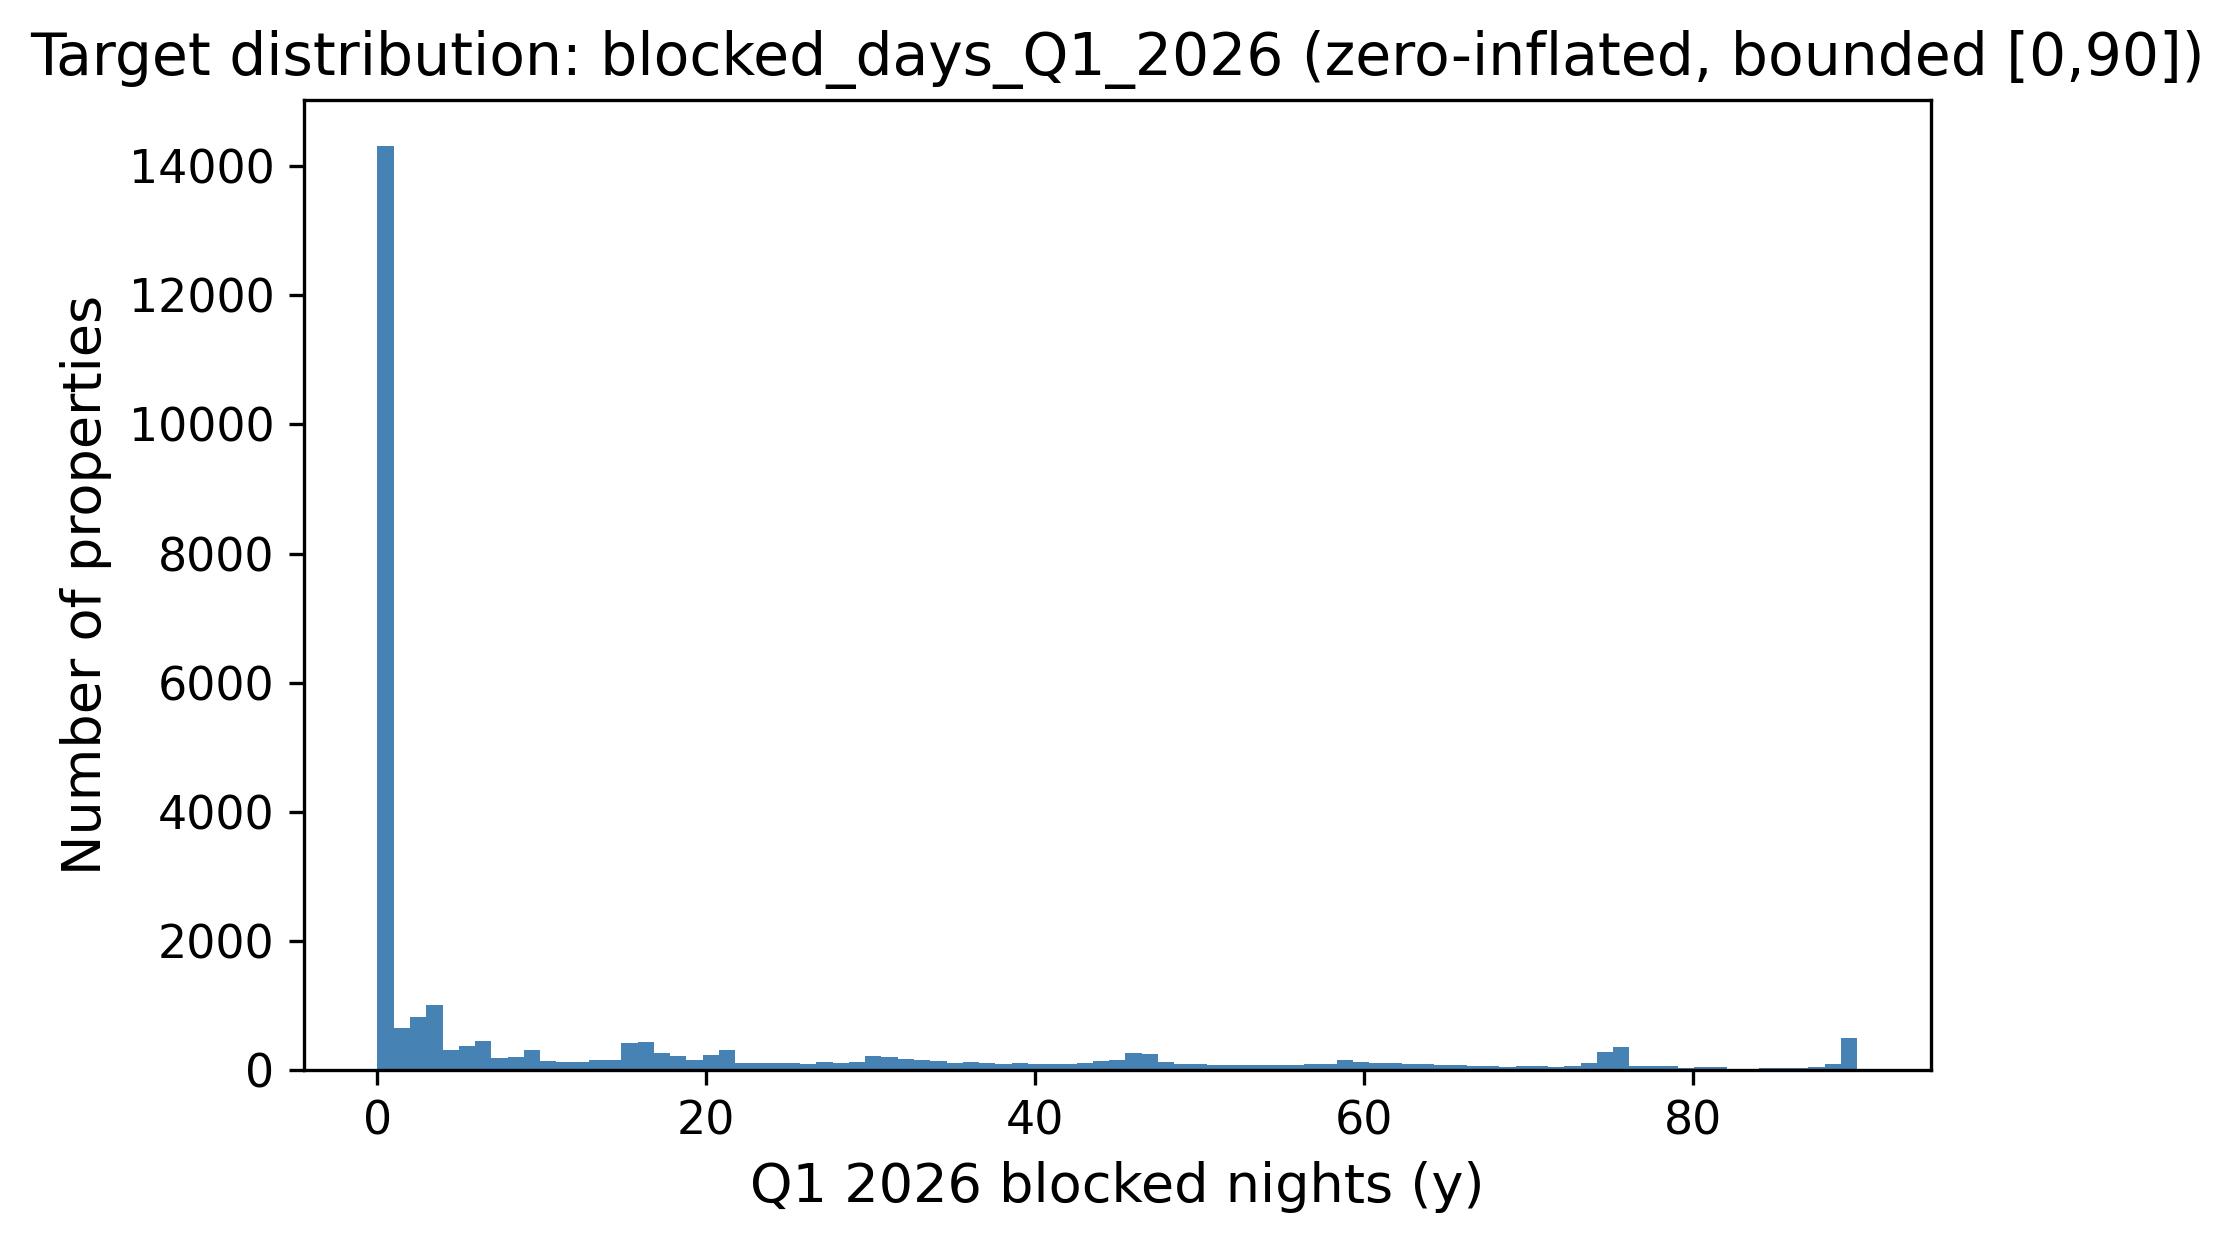
\includegraphics[width=\columnwidth]{fig1_target_dist.png}
\caption{Distribution of the target (Q1 2026 blocked nights, clean
multi-snapshot rule). The target is zero-inflated on the left and piles up
again near the 90-day maximum, which later justified clipping predictions to
$[0,90]$.}
\label{fig:target}
\end{figure}

Table~\ref{tab:targetstats} quantifies the shape of the clean target on the
full 36{,}261-listing universe. The mean (16.1) sits far above the median (1),
the distribution is strongly right-skewed (skewness $1.52$), and---most
importantly---49.6\% of properties were blocked for zero nights in Q1 2026,
while only 1.7\% reach the upper bound. This single statistic is what makes the
task a \emph{zero-inflated, bounded} regression problem rather than an ordinary
one, and it is the structural reason a least-squares estimator is biased at the
extremes (Sections~\ref{sec:linearcritique} and~\ref{sec:residuals}).
Table~\ref{tab:missing} lists the static columns with the highest missing
rates; because these are far from missing-at-random (a missing
\texttt{host\_response\_rate} typically marks an inactive host), missingness is
encoded explicitly with indicator columns rather than discarding it.

\begin{table}[!t]
\caption{Target statistics on the full listing universe ($n=36{,}261$), clean
multi-snapshot rule.}
\label{tab:targetstats}
\centering
\begin{tabular}{lc}
\toprule
Statistic & Value \\
\midrule
Mean & 16.1 \\
Median & 1 \\
Standard deviation & 25.1 \\
Skewness & 1.52 \\
Rows with $y=0$ & 49.6\% \\
Rows with $y=90$ & 1.7\% \\
\bottomrule
\end{tabular}
\end{table}

\begin{table}[!t]
\caption{Missing-value rates of the most affected static columns.}
\label{tab:missing}
\centering
\begin{tabular}{lc}
\toprule
Column & Missing rate \\
\midrule
\texttt{price} (raw) & 100\% \\
\texttt{host\_response\_rate/time} & 41.8\% \\
\texttt{beds} & 41.1\% \\
\texttt{bathrooms} & 40.8\% \\
\texttt{review\_scores\_*} & 31.3\% \\
\bottomrule
\end{tabular}
\end{table}

\subsection{Feature Engineering}
\label{sec:featuregroups}
The core of the pipeline was turning the listings snapshot and the six H2-2025
calendar/review histories into a single flat matrix with one row per listing
\texttt{id}, built strictly from data through December 2025. The result is 206
columns (205 numeric, 1 raw categorical). They fall into the following groups.
\begin{itemize}
\item \textbf{Per-quarter calendar aggregates (Q3, Q4, and combined H2).} For
each listing, the days observed, blocked, and available are counted, and
blocking/available rates are derived, separately for Q3 2025, Q4 2025, and the
combined half year, so the model sees both levels and the Q3-to-Q4 trend.
\item \textbf{Monthly blocking rates and status transitions.} The blocking
rate in each of the six individual months, plus counts of
available$\to$blocked and blocked$\to$available transitions within Q3, Q4, and
H2---a listing that changes state often is an active one.
\item \textbf{Recency and trajectory.} The same aggregates computed only over
the most recent observed window, plus a short least-squares trend fit over the
final weeks of H2, so an accelerating listing is distinguished from one that is
merely busy on average.
\item \textbf{Cross-snapshot calendar volatility.} Because Inside Airbnb
re-scrapes the same future dates every month, it is possible to observe
directly how often a listing's recorded availability for a given date
\emph{flips} between consecutive H2-2025 scrapes---this is the single strongest
predictor in the whole matrix (Fig.~\ref{fig:corr}) and has no analogue in a
dataset that supplies only one daily status per date.
\item \textbf{Price and revenue.} Price mean/min/max/range and the number of
distinct prices observed over the last five calendar snapshots, plus Airbnb's
own precomputed occupancy/revenue estimates and a price-relative-to-neighbourhood
feature; since the raw \texttt{price} column is 100\% missing in this export,
all price signal is reconstructed from the daily calendar price field.
\item \textbf{Reviews.} Review counts over 30/90/180/365-day windows and a
review-velocity acceleration term, plus the static review-score sub-ratings.
\item \textbf{Neighbourhood/geo context.} Leakage-safe context features---each
listing's neighbourhood and K-Means geo-cluster mean blocking rate and
density, computed only from the purely historical recency signal, plus the
listing's own rate relative to its neighbourhood/cluster.
\item \textbf{Property, host, and amenities.} Accommodates/bedrooms/bathrooms,
listing age, host tenure and listing-count fields, boolean host flags, and 14
binary amenity flags parsed from the JSON \texttt{amenities} column.
\item \textbf{Text keywords and property type.} Binary flags for words in the
listing title (``luxury,'' ``private,'' ``cozy,'' ``modern,'' ``view,'' etc.)
plus title length and word count, and one-hot room-/property-type groups.
\item \textbf{Raw categorical.} \texttt{neighbourhood\_cleansed} is kept as a
single raw high-cardinality categorical column and is one-hot- or
target-encoded inside each model's own cross-validation fold
(Section~\ref{sec:preproc}).
\end{itemize}

Table~\ref{tab:featgroups} summarizes the families and their sizes. The
dominant families by count are the calendar aggregates and the geography/host
blocks, but the correlation analysis (Fig.~\ref{fig:corr}) shows that raw count
does not track predictive power: the handful of cross-snapshot volatility and
recency features outweigh the much larger static-metadata block.

\begin{table}[!t]
\caption{Engineered feature families (206 columns total: 205 numeric,
1 raw categorical).}
\label{tab:featgroups}
\centering
\small
\begin{tabular}{lcp{1.15in}}
\toprule
Family & \# & Representative feature \\
\midrule
Geography (incl.\ geo-clusters) & 21 & latitude, geo\_cluster\_\{k\} \\
Host & 16 & host tenure, listing counts \\
Other property metadata & 16 & accommodates, bedrooms \\
Calendar H2 (combined) & 15 & \texttt{h2\_blocking\_rate} \\
Calendar Q3 & 14 & \texttt{q3\_blocking\_rate} \\
Amenities & 14 & \texttt{amen\_wifi}, \texttt{amen\_ac} \\
Recency window & 13 & \texttt{recent\_blocking\_rate} \\
Calendar Q4 & 12 & \texttt{q4\_blocking\_rate} \\
Text keywords & 10 & ``luxury''/``private'' flags \\
Price / revenue & 8 & \texttt{estimated\_revenue\_l365d} \\
Review scores & 8 & \texttt{review\_scores\_rating} \\
Trajectory & 7 & \texttt{traj\_slope}, \texttt{traj\_accel} \\
Property type & 7 & room-type one-hot \\
Calendar monthly & 6 & \texttt{m11\_blocking\_rate} \\
Nbhd/geo context & 6 & \texttt{nb\_mean\_rate}, \texttt{geo\_density} \\
Reviews (velocity) & 5 & \texttt{rev\_90d}, \texttt{rev\_accel\_90} \\
Borough & 5 & borough one-hot, freq.\ enc.\ \\
Cross-table ratios & 4 & \texttt{q3\_to\_q4\_blocking\_ratio} \\
Raw categorical & 1 & \texttt{neighbourhood\_cleansed} \\
\bottomrule
\end{tabular}
\end{table}

\begin{figure}[!t]
\centering
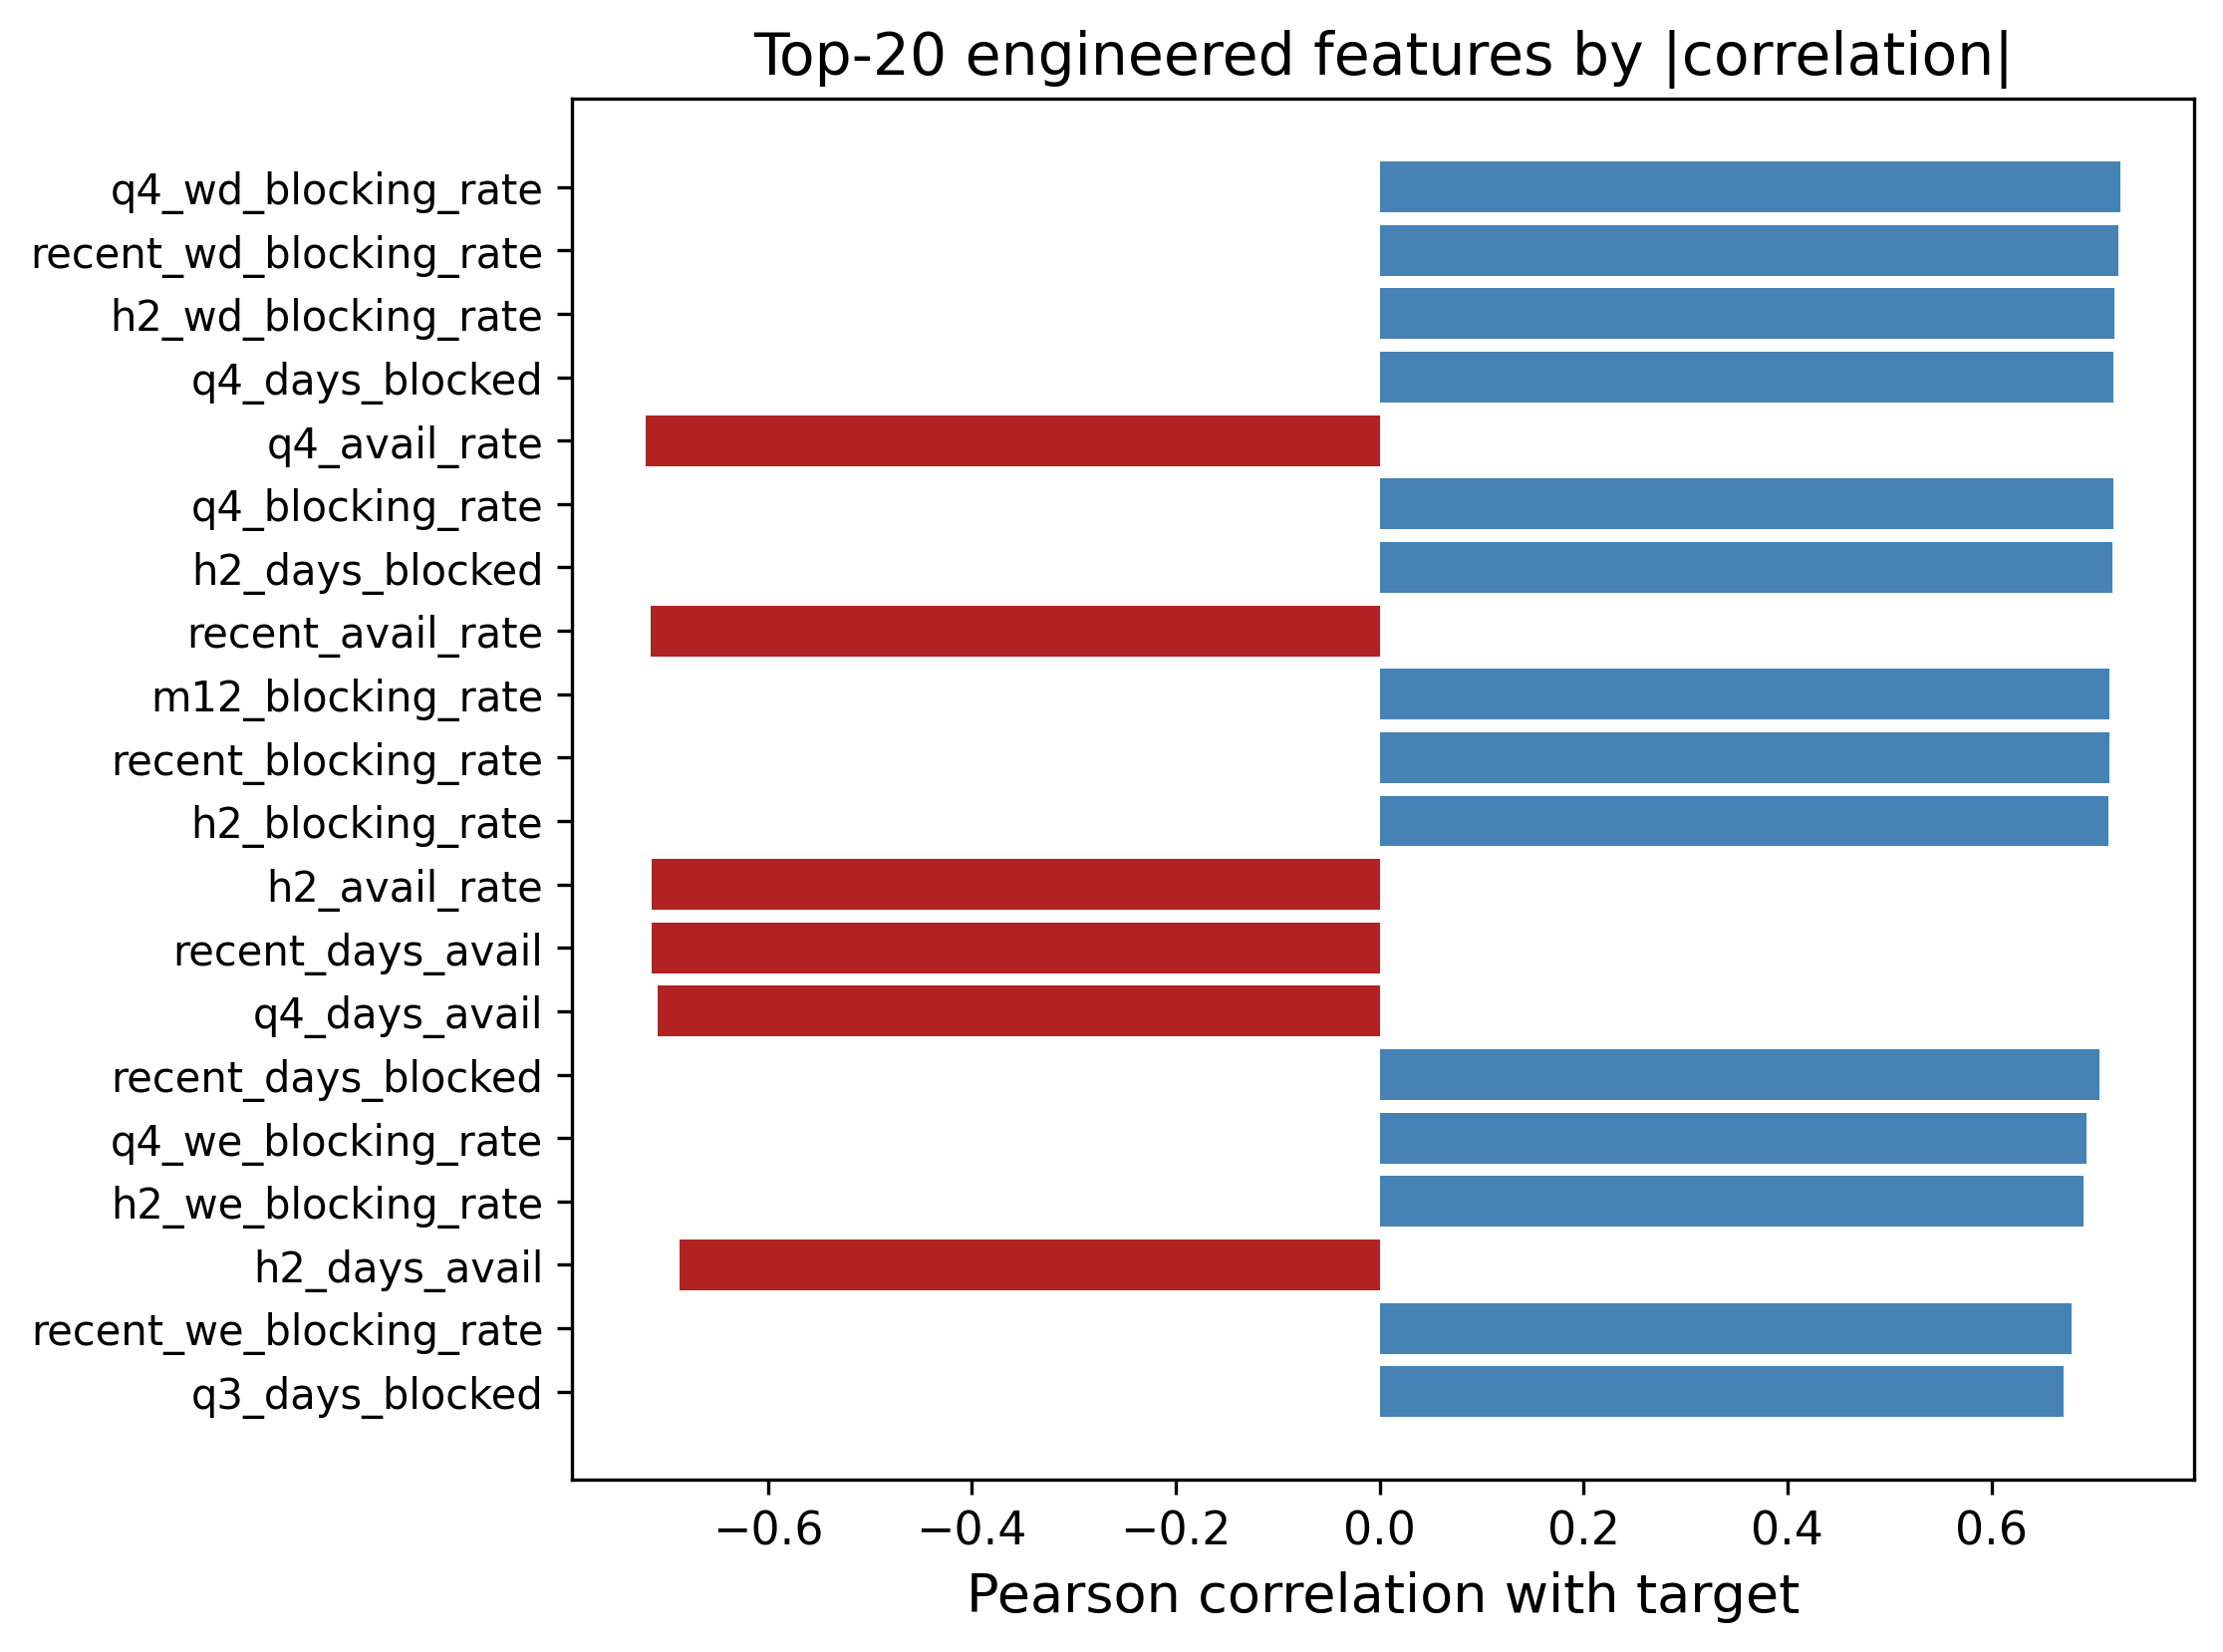
\includegraphics[width=\columnwidth]{fig2_top_corr.png}
\caption{Top engineered features by absolute correlation with the target. The
H2-2025 cross-snapshot calendar-volatility features (\texttt{h2\_flip\_rate},
\texttt{h2\_flips}) and recency/price signals dominate over static metadata.}
\label{fig:corr}
\end{figure}

\subsection{Preprocessing Pipeline and the Target Encoder}
\label{sec:preproc}
Every preprocessing step lives inside a scikit-learn \texttt{ColumnTransformer}
so that it is fit only on the training fold and then applied to the validation
fold, which keeps the workflow leakage-free. Numeric columns are
median-imputed (robust to the price outliers) with missing-indicator
columns where the missing rate is high. The one raw categorical column,
\texttt{neighbourhood\_cleansed}, is high-cardinality (well over 15 distinct
neighbourhoods), so it is handled two ways depending on the model: for Linear
Regression, Random Forest, and the MLP it is capped to its top-30 most
frequent levels (rarer levels collapse to \texttt{"Other"}) and one-hot
encoded; for the gradient-boosted models (XGBoost, LightGBM, CatBoost) a
custom $K$-fold target encoder with additive smoothing is used instead, since
trees benefit more from a single smoothed numeric column than from 30 sparse
binary ones.

\paragraph{Target-encoding formula} Let $y$ have global mean
$\mu=\tfrac{1}{n}\sum_{i=1}^{n}y_i$. For a categorical column, let level $c$
contain $n_c$ training rows with category mean
$\bar y_c=\tfrac{1}{n_c}\sum_{i:\,x_i=c}y_i$. The smoothed encoding for that
level is the count-weighted average of the category mean and the global prior,
\begin{equation}
e_c \;=\; \frac{n_c\,\bar y_c \;+\; \alpha\,\mu}{\,n_c+\alpha\,},
\qquad \alpha = 20,
\label{eq:smooth}
\end{equation}
where the smoothing factor $\alpha$ is, in effect, a number of ``pseudo-counts''
of the prior: when a level is rare ($n_c\!\ll\!\alpha$) the encoding shrinks
toward $\mu$, and when it is common ($n_c\!\gg\!\alpha$) it approaches the raw
category mean $\bar y_c$. Levels unseen at fit time map to $\mu$.

\paragraph{Leakage-free K-fold scheme} To prevent a row from informing its own
encoding, the encoder is fitted in an internal $K$-fold loop ($K=5$). Writing
$\mathcal{F}_1,\dots,\mathcal{F}_K$ for the inner folds, the encoded value of a
training row $i\in\mathcal{F}_k$ uses statistics computed \emph{only} on the
complementary folds,
\begin{equation}
\tilde e_i \;=\; e^{\,(-\mathcal{F}_k)}_{\,x_i},
\qquad i\in\mathcal{F}_k,
\label{eq:kfoldte}
\end{equation}
where $e^{\,(-\mathcal{F}_k)}_{c}$ is \eqref{eq:smooth} evaluated on
$\{(\mathbf{x}_j,y_j):j\notin\mathcal{F}_k\}$. At transform time (validation and
test rows), the full-data map is used.

To make \eqref{eq:smooth} concrete, consider a neighbourhood that appears in
$n_c=4$ training rows with a local mean of $\bar y_c=40$ blocked nights, against a
global mean of $\mu=16.1$. With $\alpha=20$ the encoded value is
$e_c=\frac{4\cdot 40+20\cdot 16.1}{4+20}=\frac{160+322}{24}\approx 20.1$, i.e.\
the estimate is pulled strongly back toward the global prior because only four
listings support it. A neighbourhood with $n_c=400$ rows and the same local mean
would instead encode to $\frac{400\cdot40+20\cdot16.1}{420}\approx 38.9$, almost
the raw mean. This shrinkage is precisely what stops rare high-cardinality levels
from injecting noisy, over-confident estimates into the model. For XGBoost, the model additionally relies on its
native missing-value handling rather than imputing, since it learns the best
split direction for NaNs on its own \cite{chen2016xgboost}. For the linear
baseline, \texttt{StandardScaler} is applied; for the tree models scaling is
unnecessary, but the rest of the pipeline is kept identical so the comparison is
fair.

\subsection{Model Selection and Rationale}
Nine model configurations from four families are compared, and a convex blend
is added on top.

\subsubsection{Linear Regression (baseline)}
A plain linear regression provides an interpretable lower bound and indicates which
features are linearly related to the target; its structural limitation on this
bounded target is analysed in Section~\ref{sec:linearcritique}.

\subsubsection{Random Forest Regressor}
A bagging ensemble \cite{breiman1996,breiman2001} that is robust to noise and
needs little tuning. It serves as a strong non-linear reference point.

\subsubsection{Gradient Boosting, XGBoost, LightGBM, and CatBoost}
Boosting builds the model sequentially and is widely regarded as the best
off-the-shelf method for tabular data \cite{friedman2001,chen2016xgboost}. A
plain scikit-learn \texttt{GradientBoostingRegressor} is trained as a weak
boosting reference, three XGBoost configurations (a hardcoded-parameter
``main'' model carried over from earlier exploration, and two independently
retuned variants, v2 and v3), and two further modern boosting libraries,
LightGBM \cite{ke2017lightgbm} and CatBoost \cite{prokhorenkova2018catboost},
are trained as additional diverse ensemble members. All of the XGBoost variants
minimize the regularized objective
\begin{equation}
\mathcal{L}(\phi)=\sum_{i=1}^{n}\ell\!\big(y_i,\hat y_i\big)
+\sum_{t}\Omega(f_t),\quad
\Omega(f)=\gamma T+\tfrac{1}{2}\lambda\lVert\mathbf{w}\rVert^{2}
+\alpha\lVert\mathbf{w}\rVert_{1},
\label{eq:xgbobj}
\end{equation}
with squared-error loss $\ell(y,\hat y)=(y-\hat y)^2$, $T$ the number of leaves,
$\mathbf{w}$ the leaf weights, and $\gamma,\lambda,\alpha$ the complexity,
$L_2$, and $L_1$ penalties. LightGBM and CatBoost optimize the same
squared-error objective with their own leaf-growth strategies, and are tuned
with the same fold-level-early-stopping search described in
Section~\ref{sec:tuning}, along with the two XGBoost variants
(Section~\ref{sec:tuning}).

\subsubsection{Multi-Layer Perceptron (MLP)}
\label{sec:mlp}
Finally, a small feed-forward neural network is trained in PyTorch
\cite{paszke2019pytorch} with the Adam optimizer \cite{kingma2015adam}. The network maps the preprocessed input
$\mathbf{z}^{(0)}=\mathbf{x}\in\mathbb{R}^{d}$ through three hidden blocks of
width $(h_1,h_2,h_3)=(256,128,64)$. Each block applies an affine map, batch
normalization, a ReLU non-linearity, and dropout with rate $p=0.2$:
\begin{align}
\mathbf{a}^{(\ell)} &= \mathbf{W}^{(\ell)}\mathbf{z}^{(\ell-1)}+\mathbf{b}^{(\ell)},
\label{eq:mlp_aff}\\
\mathbf{z}^{(\ell)} &= \mathrm{Dropout}_{p}\!\Big(\mathrm{ReLU}\big(
\mathrm{BN}(\mathbf{a}^{(\ell)})\big)\Big),\quad \ell=1,2,3,
\label{eq:mlp_block}
\end{align}
where $\mathrm{ReLU}(u)=\max(0,u)$ and batch normalization standardizes each
unit over the mini-batch $\mathcal{B}$,
\begin{equation}
\mathrm{BN}(a)=\gamma\,\frac{a-\mu_{\mathcal{B}}}{\sqrt{\sigma_{\mathcal{B}}^{2}+\epsilon}}+\beta .
\label{eq:bn}
\end{equation}
A linear read-out produces the scalar prediction in log space,
$\hat r=\mathbf{w}^{(4)\top}\mathbf{z}^{(3)}+b^{(4)}$. Because the count is
skewed, the network is trained on the log-transformed target
$t=\log(1+y)$ with the mean-squared-error criterion
$\mathcal{L}=\tfrac{1}{|\mathcal{B}|}\sum_{i\in\mathcal{B}}(\hat r_i-t_i)^2$, and
predictions are mapped back and clipped,
$\hat y=\mathrm{clip}\big(e^{\hat r}-1,\,0,\,90\big)$. Parameters are updated by
Adam with learning rate $\eta=10^{-3}$ and $L_2$ weight decay $10^{-5}$; using
the standard moment estimates $\mathbf{m}_t,\mathbf{v}_t$ of the gradient
$\mathbf{g}_t$,
\begin{equation}
\boldsymbol{\theta}_{t+1}=\boldsymbol{\theta}_{t}
-\eta\,\frac{\hat{\mathbf m}_t}{\sqrt{\hat{\mathbf v}_t}+\epsilon},
\quad
\hat{\mathbf m}_t=\frac{\mathbf m_t}{1-\beta_1^{t}},\;
\hat{\mathbf v}_t=\frac{\mathbf v_t}{1-\beta_2^{t}}.
\label{eq:adam}
\end{equation}
Training uses a batch size of 512 for up to 60 epochs with early stopping on a
held-out validation MSE (patience 8). Going in, the literature
\cite{tang2024,camatti2024} suggested the trees would win, and they
did---but the MLP turned out to be a useful blend partner because its errors
were not perfectly correlated with the trees' (Section~\ref{sec:complementarity}).

A few design choices deserve a note. Unlike the final XGBoost, the MLP is
trained on the log-transformed target $\log(1+y)$ rather than the raw count.
Neural networks are sensitive to the scale and skew of the target, and the raw
target's long right tail produced unstable gradients and slow convergence; the
log transform compresses that tail so the squared-error loss is better
conditioned, and the monotone inverse $e^{\hat r}-1$ followed by clipping returns
predictions to the count scale. This does not contradict the decision to
\emph{drop} the log transform for XGBoost (Section~\ref{sec:changes}): boosted
trees are invariant to monotone feature scaling and optimize the raw-scale loss
directly, so for them the transform only distorted the objective, whereas for the
MLP it is a numerical-stability aid. Batch normalization
\eqref{eq:bn} keeps the pre-activations well scaled across the three hidden
layers, and dropout ($p=0.2$) plus the $L_2$ weight decay in \eqref{eq:adam}
regularize a network that would otherwise overfit a 29{,}008-row table with 206
inputs.

\subsection{Hyper-Parameter Tuning}
\label{sec:tuning}
All tuning is done with 5-fold cross-validation on the 80\% development split.
For XGBoost, a custom randomized search is used instead of
\texttt{RandomizedSearchCV}, to enable fold-level early stopping: inside
each of the five outer folds, a small internal validation set is carved out, fitting
up to $B_{\max}=3000$ trees with \texttt{early\_stopping\_rounds}~$=50$, and keep
only the best iteration. \texttt{RandomizedSearchCV} does not cleanly allow a
per-fold \texttt{eval\_set} cleanly, so a custom loop was the simplest correct
option, and it also logs every configuration tried.

\paragraph{Search objective} Let $\Theta$ be the hyper-parameter space and let
the data be partitioned into outer folds $\mathcal{D}_1,\dots,\mathcal{D}_K$
($K=5$). For a configuration $\theta$, within fold $k$ the training part is split
into a fitting set and an inner validation set $\mathcal{V}_k$, grow boosting
iterations $b=1,\dots,B_{\max}$, and select the early-stopping iteration
\begin{equation}
b_k^{*}(\theta)=\operatorname*{arg\,min}_{1\le b\le B_{\max}}
\;\mathrm{RMSE}\!\Big(y^{\mathcal{V}_k},\,
\hat f^{(b)}_{\theta,k}\big(\mathbf{X}^{\mathcal{V}_k}\big)\Big),
\label{eq:earlystop}
\end{equation}
stopping once no improvement is seen for 50 consecutive rounds. The search then
minimizes the mean cross-validated MSE of the early-stopped models,
\begin{equation}
\theta^{*}=\operatorname*{arg\,min}_{\theta\in\Theta}\;
\frac{1}{K}\sum_{k=1}^{K}
\mathrm{MSE}\!\Big(y^{\mathcal{D}_k},\,
\hat f^{\,(b_k^{*}(\theta))}_{\theta,k}\big(\mathbf{X}^{\mathcal{D}_k}\big)\Big).
\label{eq:searchobj}
\end{equation}
This search is run twice for independent XGBoost variants, drawing $N=30$
configurations for ``v2'' and $N=60$ for ``v3,'' both from the product of the
marginals in Table~\ref{tab:search}, sampling the learning rate and the
regularization terms log-uniformly so that small and large scales are explored
evenly, as recommended by \cite{bergstra2012random}. The full procedure is
summarized in Algorithm~1. LightGBM and CatBoost are tuned with the same
fold-level-early-stopping principle over $N=40$ draws each, but over their own
native parameter spaces. The ``main'' XGBoost configuration (used in the
baseline comparison of Table~\ref{tab:cv}) instead carries fixed, hand-set
hyper-parameters from earlier exploratory runs, with no independent search or
early stopping of its own in this iteration of the pipeline; comparing its
score to the independently-tuned v2/v3 variants (Table~\ref{tab:metrics}) is
itself an informal check on how much headroom the search actually finds.

\begin{table}[!t]
\caption{Search distributions for the randomized search (used for both the v2
and v3 XGBoost variants). $\mathrm{LogU}$ denotes a log-uniform draw,
$\mathcal{U}$ a uniform draw.}
\label{tab:search}
\centering
\begin{tabular}{ll}
\toprule
Hyper-parameter & Sampling distribution \\
\midrule
\texttt{n\_estimators} (cap $B_{\max}$) & $3000$ (fixed) \\
\texttt{learning\_rate} & $\mathrm{LogU}(0.02,\,0.10)$ \\
\texttt{max\_depth} & $\mathcal{U}\{4,\dots,8\}$ \\
\texttt{min\_child\_weight} & $\mathcal{U}\{1,\dots,11\}$ \\
\texttt{subsample} & $\mathcal{U}(0.65,\,0.95)$ \\
\texttt{colsample\_bytree} & $\mathcal{U}(0.65,\,0.95)$ \\
\texttt{gamma} ($\gamma$) & $\mathcal{U}(0.0,\,0.4)$ \\
\texttt{reg\_alpha} ($\alpha$) & $\mathrm{LogU}(10^{-3},\,0.5)$ \\
\texttt{reg\_lambda} ($\lambda$) & $\mathrm{LogU}(0.5,\,5.0)$ \\
\bottomrule
\end{tabular}
\end{table}

\vspace{2pt}
\noindent\textbf{Algorithm 1: Randomized search with fold-level early stopping.}
\emph{Input:} hyper-parameter space $\Theta$, outer folds
$\{\mathcal{D}_k\}_{k=1}^{K}$, budget $N$, tree cap $B_{\max}$.
\begin{enumerate}
\item Initialize $\theta^{*}\leftarrow\varnothing$, $s^{*}\leftarrow+\infty$.
\item For $j=1,\dots,N$: sample a configuration $\theta\sim\Theta$ from
Table~\ref{tab:search}.
\item For each fold $k=1,\dots,K$: fit the preprocessing on the training part,
carve an inner validation set $\mathcal{V}_k$, grow up to $B_{\max}$ trees, pick
the early-stop iteration $b_k^{*}$ by \eqref{eq:earlystop}, and record
$m_k=\mathrm{MSE}$ on $\mathcal{D}_k$ using $b_k^{*}$ trees.
\item Set $s=\frac{1}{K}\sum_k m_k$ and log $(\theta,s)$; if $s<s^{*}$, update
$s^{*}\leftarrow s$, $\theta^{*}\leftarrow\theta$.
\item After $N$ configurations, return $\theta^{*}$.
\end{enumerate}
\vspace{2pt}

The best v3 configuration (Table~\ref{tab:xgbparams}) uses a learning rate of
0.026, max depth 8, subsample 0.80, and \texttt{colsample\_bytree} 0.68, and
early stopping settled around 363 trees on average -- despite a search cap of
3{,}000, none of the 60 configurations needed anywhere near that many
iterations before its held-out validation error stopped improving. The v2
search (30 configurations) converges to an almost identical region (learning
rate 0.025, max depth 8, $\approx$363 trees) and a nearly identical score
(Table~\ref{tab:metrics}), a useful sanity check that two independent searches
over the same space land in the same neighbourhood rather than at different
local optima.

\begin{table}[!t]
\caption{Best XGBoost (v3) hyper-parameters found by the 60-configuration
randomized search.}
\label{tab:xgbparams}
\centering
\begin{tabular}{ll}
\toprule
Hyper-parameter & Value \\
\midrule
\texttt{n\_estimators} (cap) & 3000 \\
\texttt{learning\_rate} & 0.0262 \\
\texttt{max\_depth} & 8 \\
\texttt{min\_child\_weight} & 3 \\
\texttt{subsample} & 0.804 \\
\texttt{colsample\_bytree} & 0.680 \\
\texttt{gamma} & 0.314 \\
\texttt{reg\_alpha} & 0.0158 \\
\texttt{reg\_lambda} & 3.244 \\
\texttt{early\_stopping\_rounds} & 50 ($\approx$363 trees kept) \\
\bottomrule
\end{tabular}
\end{table}

\noindent\emph{Note.} The independently-tuned search (295.8 CV MSE for v3,
Table~\ref{tab:metrics}) essentially matches, rather than clearly beats, the
hand-set ``main'' XGBoost configuration (295.7 CV MSE) carried over from
earlier exploration without a dedicated search of its own. This is read as an
informative negative result rather than a wasted search: on this feature set,
a reasonably-chosen manual configuration and a 30--60 iteration randomized
search reach comparable error, suggesting the ceiling here is set more by the
feature matrix than by exact tree hyper-parameters (Section~\ref{sec:ablation}).

\subsection{Ensembling (Weighted Blend)}
\label{sec:blend}
Rather than using a single model, the out-of-fold (OOF) predictions are combined
of the candidate models with a convex weighted average. Stack the $m$ models'
OOF predictions into a matrix $\mathbf{P}\in\mathbb{R}^{n\times m}$ with column
$j$ holding model $j$'s OOF prediction. The aim is to find weights
$\mathbf{w}\in\mathbb{R}^{m}$ that minimize the blended MSE, subject to the
predictions staying on the valid scale:
\begin{align}
\min_{\mathbf{w}\in\mathbb{R}^{m}}\quad
& \frac{1}{n}\sum_{i=1}^{n}\Big(y_i-\mathrm{clip}\big[(\mathbf{P}\mathbf{w})_i,\,0,\,90\big]\Big)^{2}
\label{eq:blendobj}\\
\text{s.t.}\quad & \sum_{j=1}^{m}w_j = 1,
\label{eq:blendeq}\\
& 0 \le w_j \le 1,\quad j=1,\dots,m.
\label{eq:blendbox}
\end{align}
The equality constraint~\eqref{eq:blendeq} and the box
bounds~\eqref{eq:blendbox} make the solution a \emph{convex combination}, which
keeps the blend on the same scale as the inputs and prevents any single model
from receiving a runaway weight. Problem \eqref{eq:blendobj}--\eqref{eq:blendbox} is solved
with Sequential Least-Squares Quadratic Programming (SLSQP) via
\texttt{scipy.optimize.minimize}, starting from the uniform point
$w_j^{(0)}=1/m$ with \texttt{ftol}~$=10^{-9}$. As a post-processing step, weights below $10^{-4}$
are zeroed and the rest renormalized so that
\eqref{eq:blendeq} still holds exactly. A randomized search directly over the
weight simplex is also run as a sanity check and yields the same optimum,
confirming the SLSQP solution is not an artefact of that particular optimizer.
Across the nine candidate models, the optimizer concentrated most of the
weight on the main XGBoost ($\approx0.45$), with substantial secondary weight
on LightGBM ($\approx0.18$) and Random Forest ($\approx0.16$), smaller
contributions from XGBoost v3 ($\approx0.10$), CatBoost ($\approx0.07$), and
the MLP ($\approx0.05$), a negligible weight on XGBoost v2 ($\approx0.004$),
and Linear Regression and the plain Gradient Boosting baseline dropped to zero
(Table~\ref{tab:weights}). The full procedure is given in Algorithm~2.

\vspace{2pt}
\noindent\textbf{Algorithm 2: Convex weighted blend via SLSQP.}
\emph{Input:} OOF matrix $\mathbf{P}\in\mathbb{R}^{n\times m}$, targets
$\mathbf{y}$.
\begin{enumerate}
\item Define the objective
$g(\mathbf{w})=\frac{1}{n}\lVert\mathbf{y}-\mathrm{clip}(\mathbf{P}\mathbf{w},0,90)\rVert_2^2$.
\item Initialize $\mathbf{w}^{(0)}=(1/m,\dots,1/m)$.
\item Minimize $g$ with SLSQP subject to $\sum_j w_j=1$ and $0\le w_j\le1$ to
obtain $\mathbf{w}^{*}$.
\item Prune: set $w_j^{*}=0$ for every $j$ with $w_j^{*}<10^{-4}$.
\item Renormalize $\mathbf{w}^{*}\leftarrow\mathbf{w}^{*}/\sum_j w_j^{*}$ and
return $\mathbf{w}^{*}$.
\end{enumerate}
\vspace{2pt}

\subsection{Experimental Design and Evaluation}
The labelled data are split once into an 80\% development set (29{,}008
properties) and a 20\% local hold-out (7{,}253 properties) with a fixed seed,
so every model is trained and selected on exactly the same rows, and the
hold-out is touched only for the final numbers in Section~\ref{sec:results}.
Inside the development set, 5-fold cross-validation is used for both model
selection and tuning. MSE is optimised directly, while MAE and $R^2$ are also
tracked internally because they are easier to read. To prevent leakage, (i)
every preprocessing step is fitted only on the training fold, (ii) no feature
is built from any 2026 information (Section~\ref{sec:dataset}), and (iii)
target encodings are computed inside their own inner $K$-fold per
\eqref{eq:kfoldte}. As a last step, predictions are clipped to $[0,90]$, both
because no property can be blocked more than 90 nights in a 90-day quarter and
to bound the loss contributed by any stray extrapolation.

\subsection{Computational Cost}
\label{sec:cost}
Because the experiments ran on a single workstation rather than a cluster,
computational cost was monitored throughout. Building the 206-feature matrix
from the 79 million H2-2025 calendar/review rows is a one-time aggregation
that dominates wall-clock time but is trivially parallelizable over listings.
Model training is cheap by comparison: a single early-stopped XGBoost fit
converges at $\approx$363 trees on average, so the 60-configuration v3 search
and the 30-configuration v2 search (Algorithm~1) each complete in well under an
hour on commodity hardware (Appendix~A). The Random Forest, LightGBM, and
CatBoost searches are of the same order; the linear, MLP, and plain
gradient-boosting baselines are faster still. The SLSQP blend itself is
essentially free---it optimizes only $m=9$ weights over a fixed $n\times m$
matrix of cached OOF predictions, converging in well under a second. This
favourable cost profile is one practical reason a small, well-tuned ensemble is
preferred over a single very large model: the marginal compute of adding the
blend is negligible relative to the searches, yet it returns a statistically
significant accuracy gain (Section~\ref{sec:significance}).

\subsection{Reproducibility and Implementation}
\label{sec:repro}
Every result in this paper is reproducible from a single fixed seed
(\texttt{random\_state}~$=42$), which governs the 80/20 development/hold-out
split, the 5-fold cross-validation partitions, the inner target-encoding folds,
and the random-search samplers. The pipeline is implemented entirely in Python
with scikit-learn \cite{pedregosa2011sklearn} for the preprocessing
\texttt{ColumnTransformer}, imputers, one-hot encoder, linear, random-forest and
gradient-boosting models and cross-validation; the \texttt{xgboost}
\cite{chen2016xgboost}, \texttt{lightgbm} \cite{ke2017lightgbm}, and
\texttt{catboost} \cite{prokhorenkova2018catboost} packages for the boosted
trees; PyTorch \cite{paszke2019pytorch} with Adam \cite{kingma2015adam} for the
MLP; and \texttt{scipy.optimize} for the SLSQP blend. The code is organized as
a sequence of numbered notebooks---exploratory analysis, feature engineering,
one notebook per model family (including three XGBoost variants and a
dedicated hurdle-model notebook), the blend, an incremental ablation, and a
figures notebook---so that each stage can be re-run independently, and the
out-of-fold predictions are cached to disk (\texttt{.npy}) so that the blend
and all of the post-hoc diagnostics in Section~\ref{sec:results} can be
recomputed without retraining.

%==============================================================================
\section{Results and Discussion}
\label{sec:results}
Table~\ref{tab:cv} lists the 5-fold cross-validation scores of all nine model
configurations on the development set, including two strong external
gradient-boosting baselines. The ordering is consistent with the literature.
Linear Regression and the untuned Gradient Boosting trail the field, Random
Forest and the MLP sit in the middle, and the boosted-tree family (XGBoost and
its variants, LightGBM, CatBoost) clusters tightly at the top, all within about
2 MSE points of one another. The hand-set main XGBoost configuration (295.7)
and the independently 60-configuration-tuned XGBoost v3 (295.8) are
statistically indistinguishable, and the SLSQP blend of all nine models lowers
the out-of-fold error to 290.1---about a $1.9\%$ relative improvement over the
best single model.

Crucially, the proposed pipeline is also benchmarked against two
state-of-the-art gradient-boosting libraries widely used in tabular
forecasting, LightGBM and CatBoost, trained with the same leakage-safe
preprocessing and the same 5-fold split. As reported in Table~\ref{tab:cv},
tuned LightGBM (296.5) and CatBoost (301.5) are competitive but do \emph{not}
clearly surpass the in-house tuned XGBoost variants ($\approx$295.7--295.8),
and all are behind the convex blend (290.1). This shows that the reported
gains stem from the temporal feature engineering, the leakage-safe target
encoding, and the optimized convex ensemble rather than from the choice of a
particular boosting library.

\begin{table}[!t]
\caption{Model comparison by 5-fold CV on the development set (29{,}008
properties; lower MSE/MAE and higher $R^2$ are better). LightGBM and CatBoost
are state-of-the-art external baselines trained with the identical pipeline.}
\label{tab:cv}
\centering
\begin{tabular}{lccc}
\toprule
Model & MSE & MAE & $R^2$ \\
\midrule
LinearRegression & 357.6 & 12.24 & 0.432 \\
GradientBoosting & 435.8 & 11.04 & 0.308 \\
RandomForest & 302.8 & 10.32 & 0.519 \\
MLP & 382.5 & 10.40 & 0.393 \\
\midrule
LightGBM (SOTA baseline) & 296.5 & 10.20 & 0.529 \\
CatBoost (SOTA baseline) & 301.5 & 10.43 & 0.522 \\
XGBoost v2 (retuned) & 296.9 & 10.21 & 0.529 \\
XGBoost v3 (retuned) & 295.8 & 10.18 & 0.531 \\
XGBoost (main, proposed) & 295.7 & 10.05 & 0.531 \\
\textbf{SLSQP weighted blend (proposed)} & \textbf{290.1} & \textbf{10.02} & \textbf{0.540} \\
\bottomrule
\end{tabular}
\end{table}

\begin{figure}[!t]
\centering
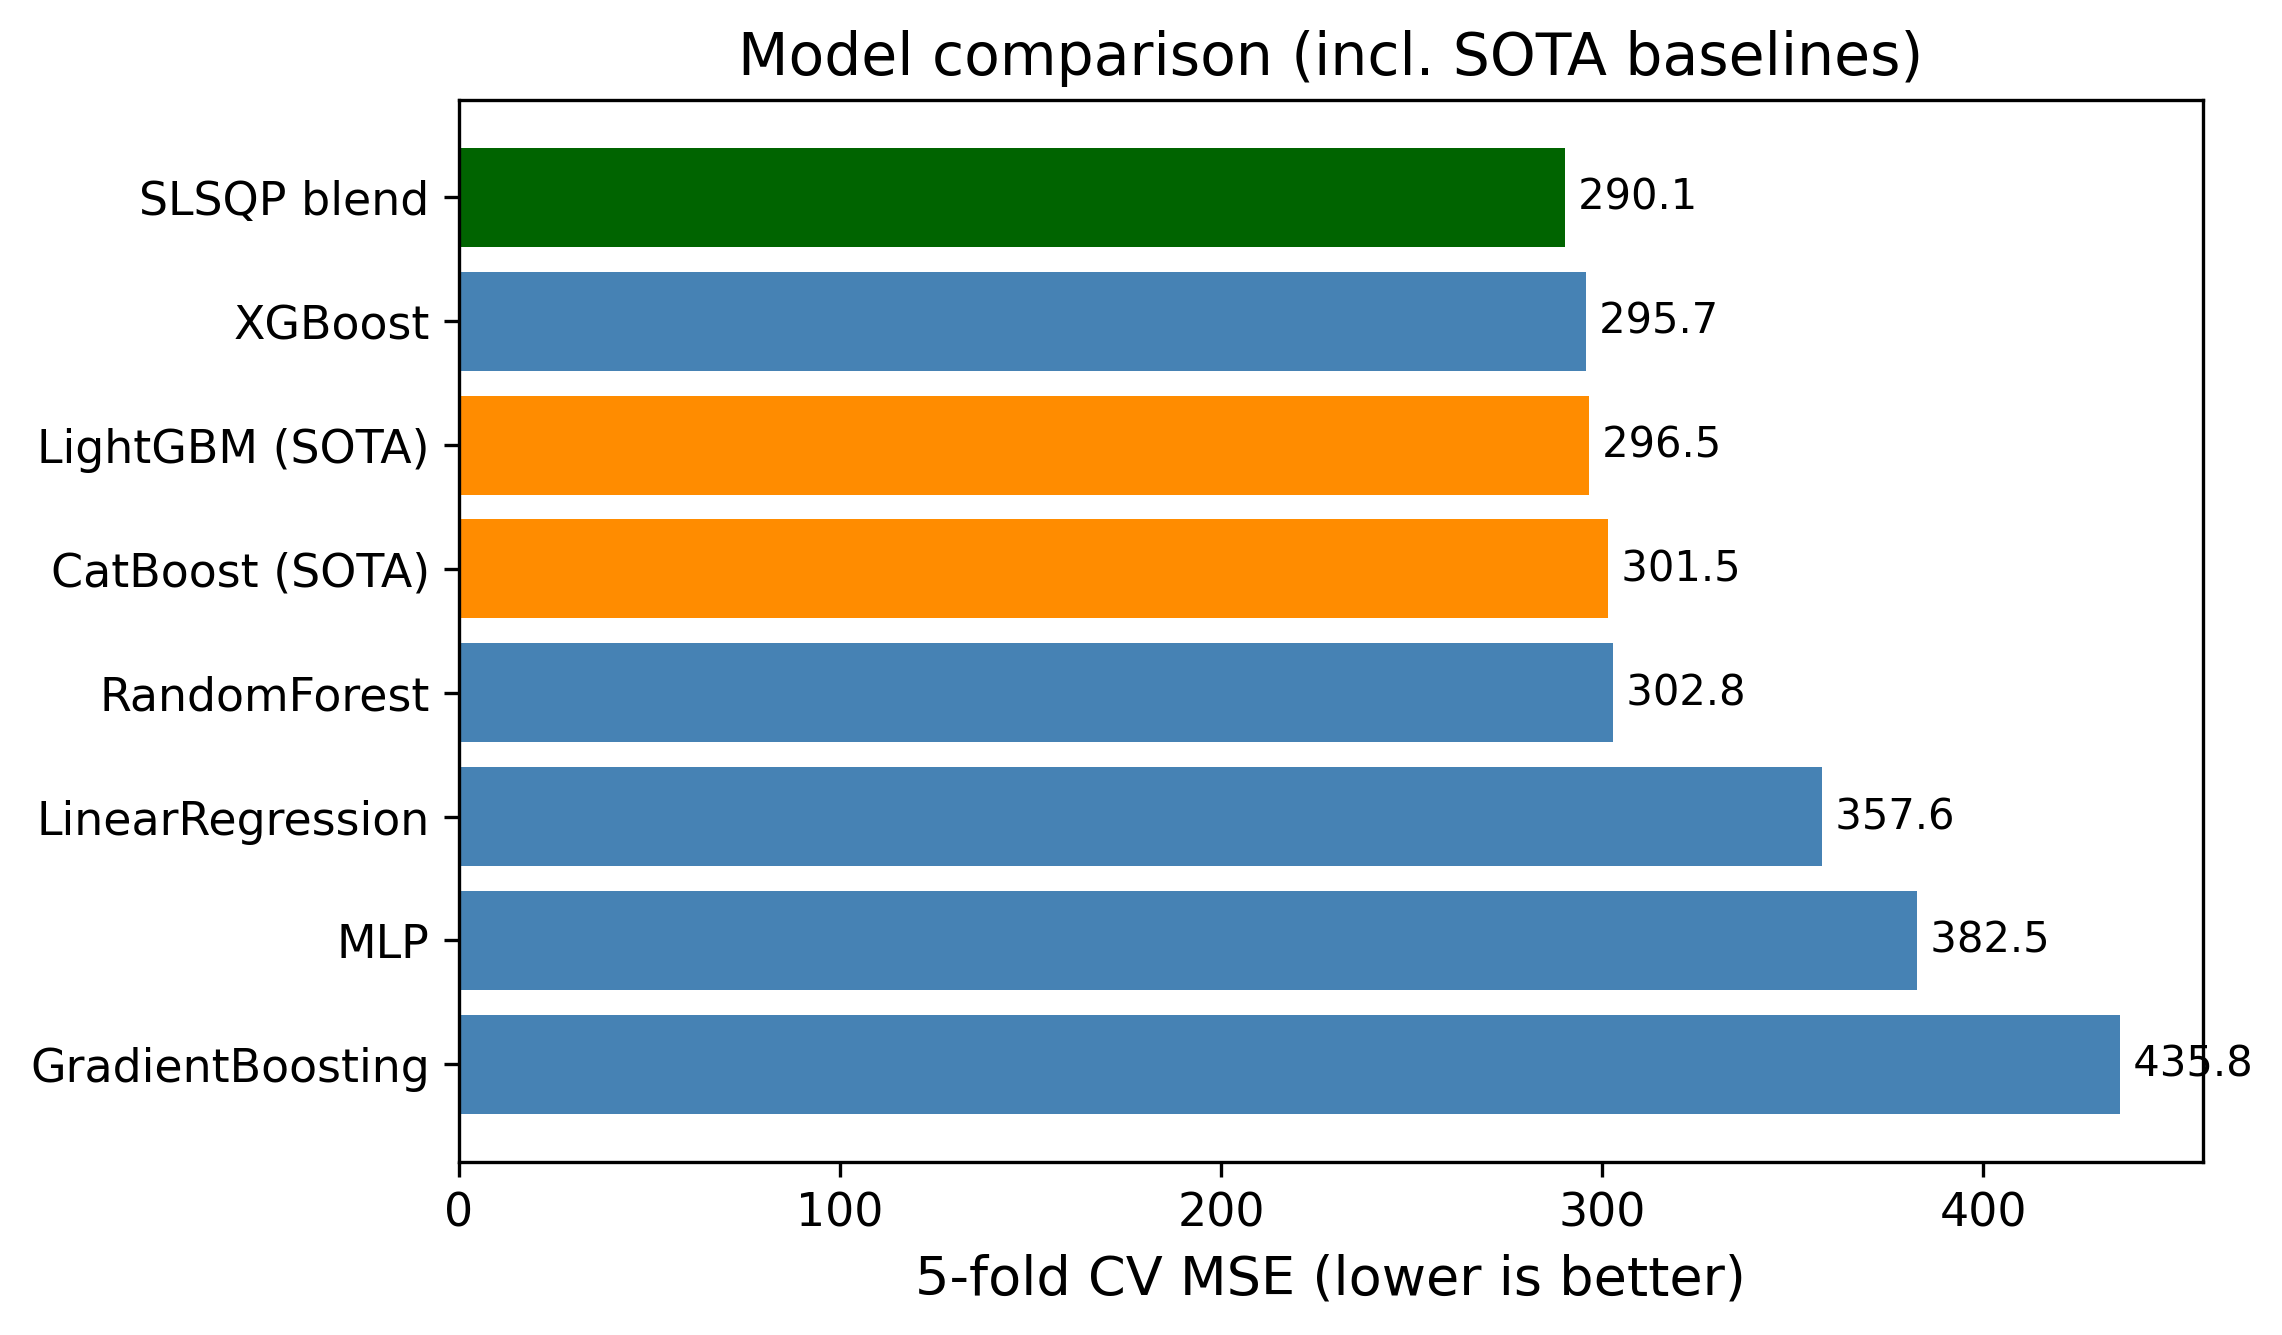
\includegraphics[width=\columnwidth]{fig3_baseline_cv.png}
\caption{Model comparison by cross-validated MSE, including the LightGBM/
CatBoost baselines and the final blend. The tree-based models cluster tightly
at the top; Linear Regression, the MLP, and the untuned Gradient Boosting
trail well behind.}
\label{fig:baseline}
\end{figure}

\subsection{Why the Methods Behaved as They Did}
The gap between the linear model and the boosted trees is the clearest result,
and it is exactly the structural mismatch made precise in
Section~\ref{sec:linearcritique}: the relationship between the features and the
bounded, zero-inflated target is strongly non-linear and full of
interactions---for example, a high H2-2025 blocking rate means something very
different for a listing whose calendar has been flipping back and forth every
month than for one that has been stably booked. Linear regression cannot
represent those interactions without hand-crafting them, while trees discover
them automatically. Random Forest captures the non-linearity but, being a
variance-reduction (bagging) method, it cannot reduce bias as aggressively as
boosting can. The boosted-tree family combines low bias (sequential residual
fitting) with strong regularization and, for the tuned variants, early
stopping, which is why that whole family clusters at the top. The MLP landed
between the trees and the linear model; neural networks usually need more data
and more careful tuning to beat gradient boosting on tabular problems, and the
compute budget did not allow a deep search.

It is useful to read the whole ranking through a bias--variance lens. Linear
regression is a high-bias, low-variance estimator: it cannot bend to the
saturating conditional mean of Section~\ref{sec:linearcritique}, so its error is
dominated by bias and no amount of data removes it. Random Forest attacks the
opposite term---bagging averages many high-variance trees to cut variance---but,
because every tree is grown to near-purity on the same features, it leaves a
residual bias that boosting can still reduce. Gradient boosting lowers bias by
fitting residuals stage by stage, and the tuned boosted-tree models add the
regularization and early stopping \eqref{eq:xgbobj}--\eqref{eq:earlystop} that
keep the corresponding variance in check, which is why they sit at the bottom
of the MSE column. The MLP is capable of low bias in principle, but on
29{,}008 rows it is variance-limited without heavier regularization, which is
exactly why batch normalization and dropout (Section~\ref{sec:mlp}) mattered so
much to its stability. The blend then performs one more variance reduction
\emph{across} model families rather than within one, which is why it improves
on even the best single model.

\begin{figure}[!t]
\centering
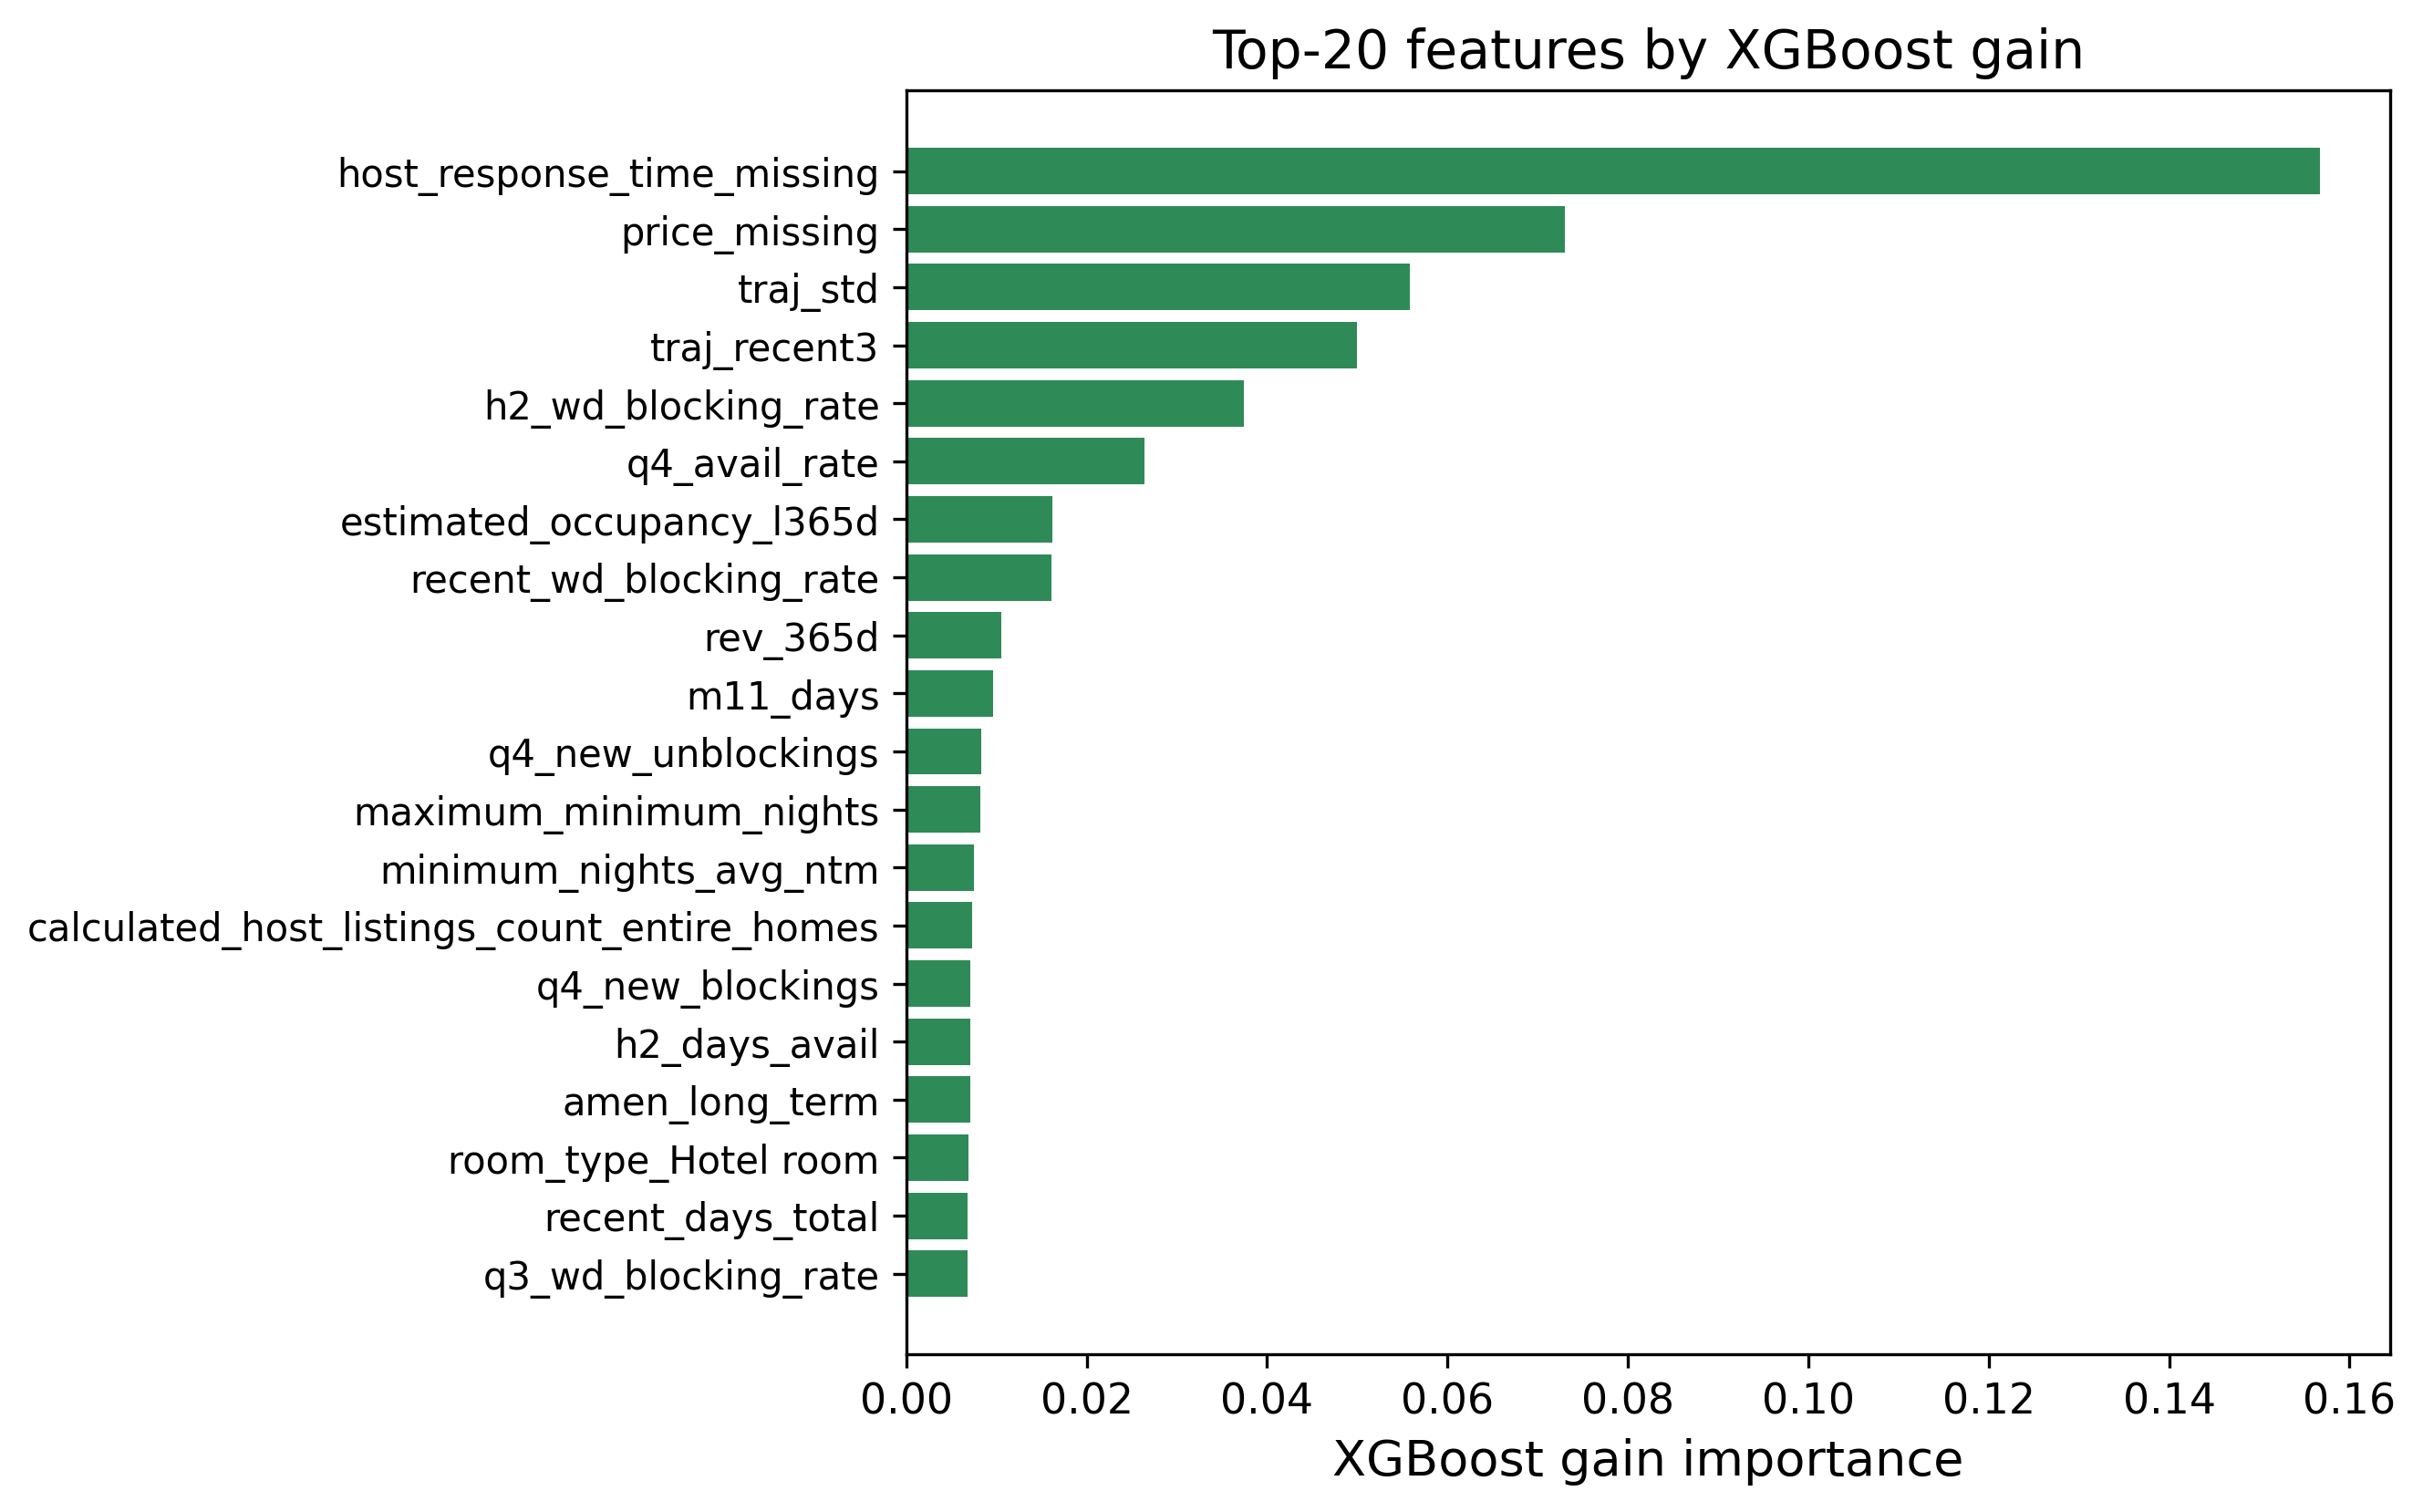
\includegraphics[width=\columnwidth]{fig4_xgb_importance.png}
\caption{XGBoost gain-based feature importances. The H2-2025 calendar-volatility
features dominate, in agreement with Fig.~\ref{fig:corr}.}
\label{fig:importance}
\end{figure}

The feature-importance analysis (Fig.~\ref{fig:importance}) confirms the EDA
story: the model leans most heavily on \texttt{h2\_flip\_rate} (by a wide
margin), the H2 weekday blocking rate, the missing-host-response-time and
missing-price indicators, and the recency-window features, with most of the
static metadata and text keywords playing only a supporting role. This is
reassuring because it means the model is using genuine calendar-behaviour
signals rather than spurious artefacts, and it illustrates a broader point from
Section~\ref{sec:lit}: the single feature that matters most exists only
because this dataset's repeated monthly re-scrapes make it observable.

\subsection{Impact of the Blend and the Optimization Choices}
Two optimization decisions mattered most for the final score. The first was
early stopping: letting each fold stop when its internal validation error
stopped improving, rather than growing a fixed number of trees, gave the
independently-tuned variants most of the benefit of a large ensemble without
the overfitting risk, and made the searches cheaper because bad configurations
stopped early. The second was the blend. An equal-weight average of all nine
models scored 301.0 OOF, which is \emph{worse} than the best single model
(295.7), because the weak models drag it down. Once SLSQP chooses the weights,
the error drops to 290.1---the optimizer effectively down-weighted the weak
models and concentrated weight on the complementary tree ensembles.
Fig.~\ref{fig:blend} shows the per-model and blended OOF scores side by side, and
Table~\ref{tab:weights} lists the optimal weights.

\begin{figure}[!t]
\centering
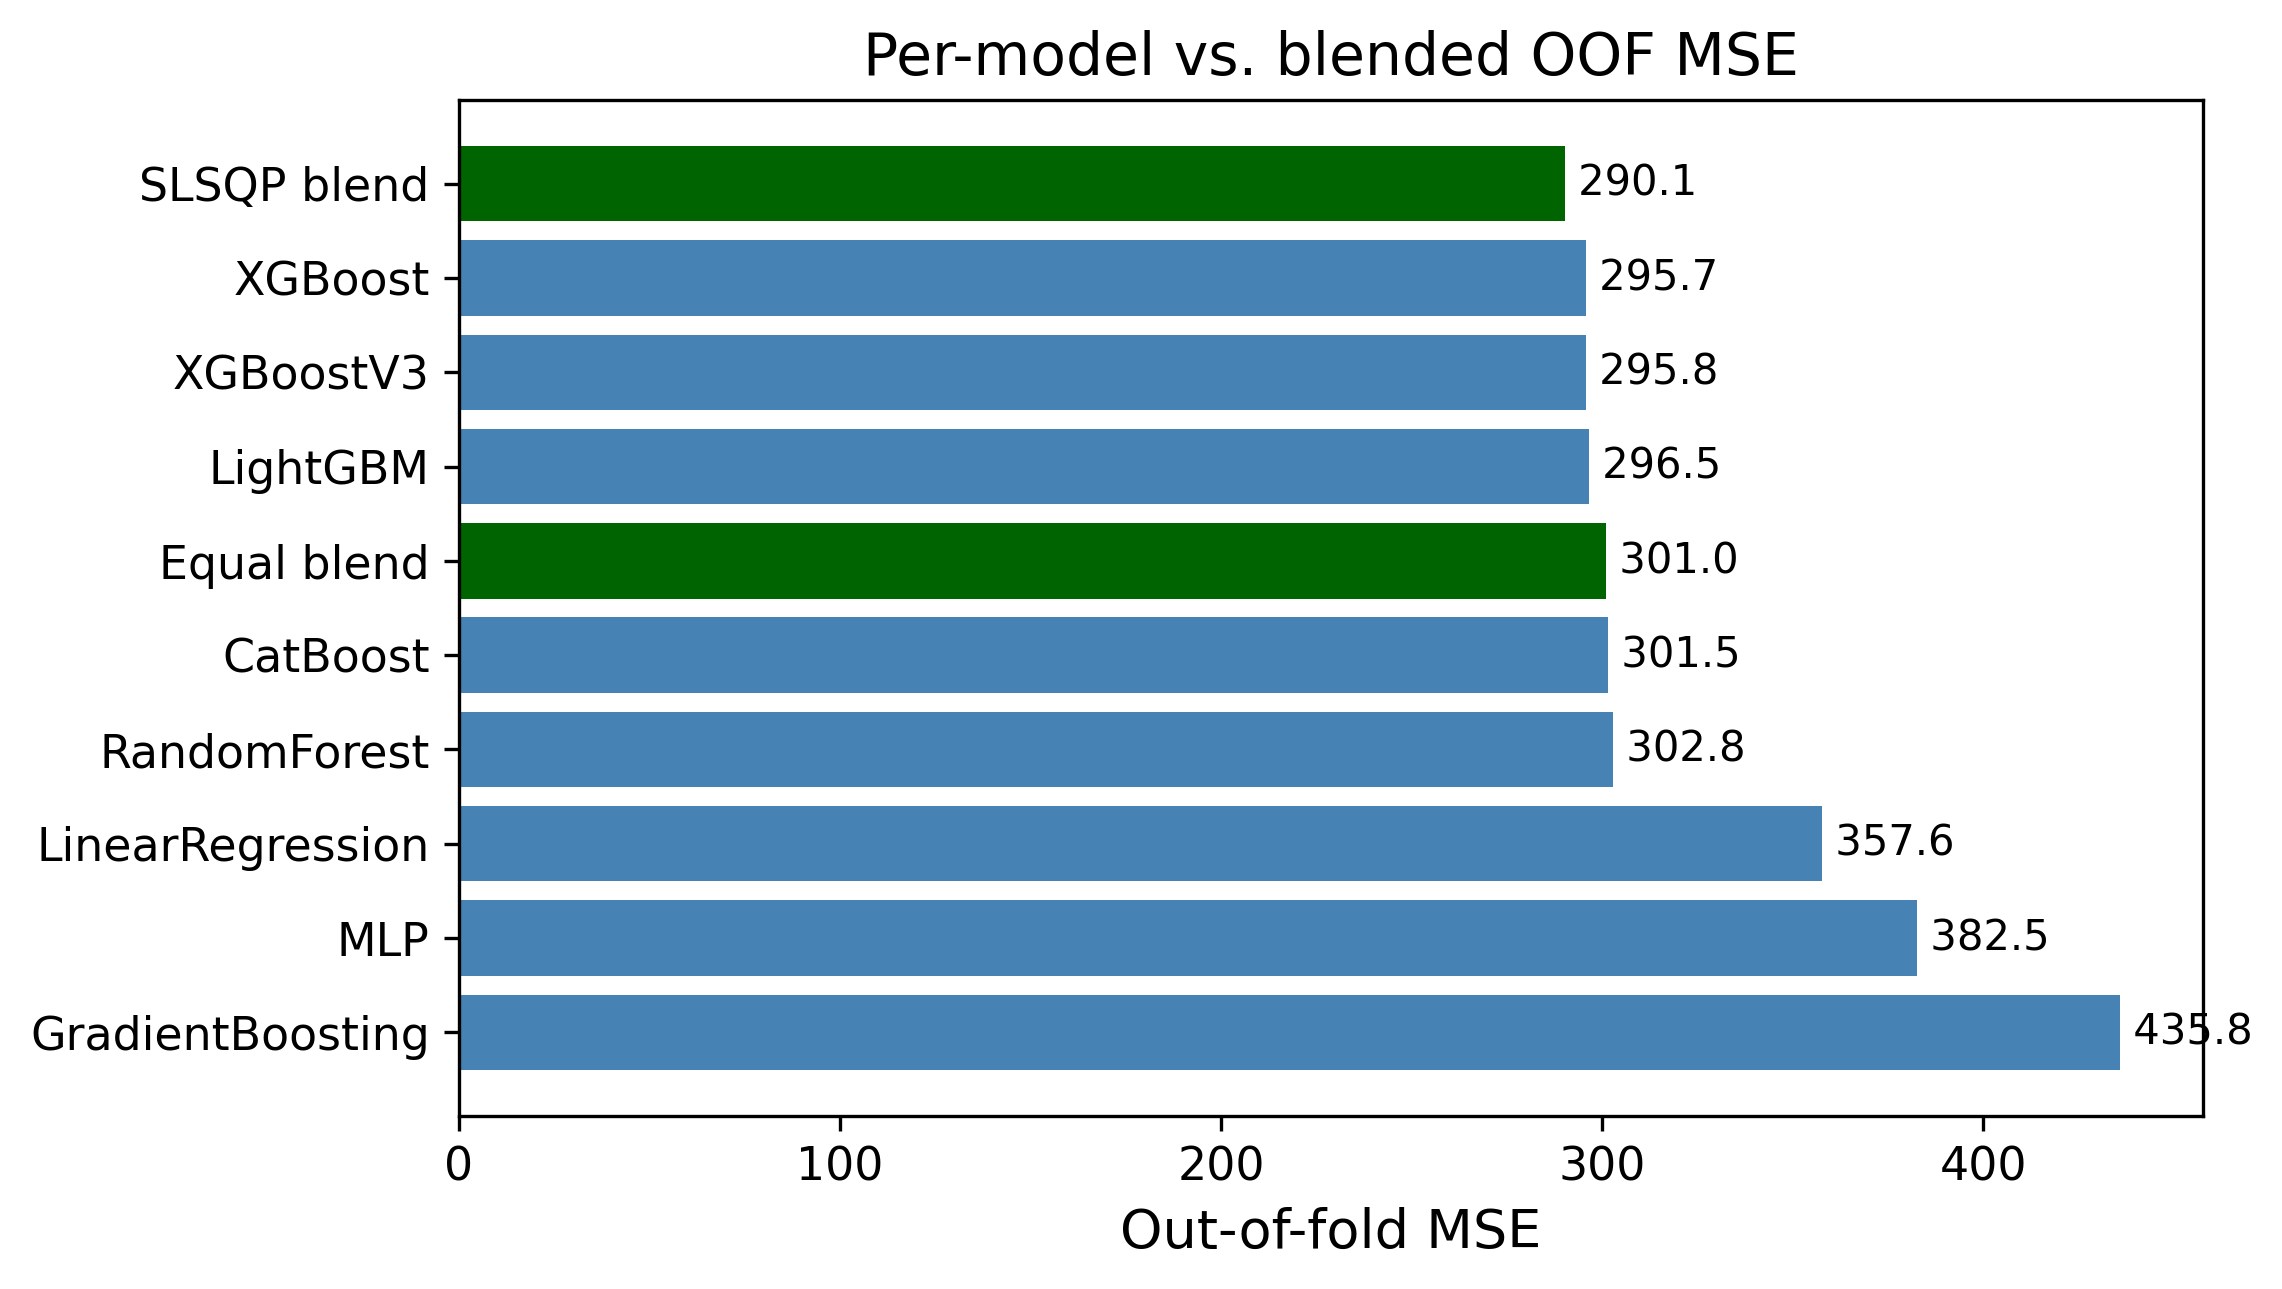
\includegraphics[width=\columnwidth]{fig5_blend.png}
\caption{Out-of-fold MSE for each model and for the equal-weight vs.\ optimal
(SLSQP) blends. The weighted blend is the best configuration.}
\label{fig:blend}
\end{figure}

\begin{table}[!t]
\caption{Optimal blend weights chosen by SLSQP on the OOF predictions of all
nine models (problem~\eqref{eq:blendobj}--\eqref{eq:blendbox}).}
\label{tab:weights}
\centering
\begin{tabular}{lc}
\toprule
Model & Weight $w_j$ \\
\midrule
XGBoost (main) & 0.4450 \\
LightGBM & 0.1782 \\
RandomForest & 0.1585 \\
XGBoost v3 & 0.0957 \\
CatBoost & 0.0682 \\
MLP & 0.0502 \\
XGBoost v2 & 0.0041 \\
LinearRegression & 0.0000 \\
GradientBoosting & 0.0000 \\
\bottomrule
\end{tabular}
\end{table}

\subsection{Model Complementarity and Final Error Metrics}
\label{sec:complementarity}
A blend can only help if its members make \emph{different} mistakes; if every
model erred on the same rows, averaging them would just reproduce the common
error. Table~\ref{tab:errcorr} reports the Pearson correlation of the per-row
prediction errors across all nine models. All of the tree models are highly
correlated with one another (most pairwise correlations above $0.95$), which is
why the optimizer keeps only three of the six boosted-tree/forest variants at
meaningful weight and drives XGBoost v2 and Gradient Boosting essentially to
zero (Table~\ref{tab:weights}) despite XGBoost v2 individually outscoring
several models that do receive weight---it largely duplicates signal already
covered by the main XGBoost and v3. The MLP and Linear Regression are the
least correlated with the tree ensembles ($0.86$--$0.93$ with the others), so
although they are individually much weaker (Table~\ref{tab:metrics}), the MLP
still carries enough independent signal to receive a small supporting weight,
while Linear Regression's error turns out to be fully explained by the
stronger models and is dropped to zero. This is the quantitative justification
for the weight pattern in Table~\ref{tab:weights}: SLSQP is not merely picking
the best models, it is exploiting error de-correlation.

Table~\ref{tab:metrics} also reports the blend's MAE and $R^2$ alongside MSE.
The blend improves not only the optimized MSE (290.13 vs.\ 295.73 for the best
single model) but also the $R^2$ (0.540 vs.\ 0.531), and its MAE (10.02) beats
every individual model's MAE as well---so the MSE gain does not come at the
cost of median accuracy.

\begin{table}[!t]
\caption{Final error metrics on the development OOF predictions (lower MSE/MAE,
higher $R^2$ are better).}
\label{tab:metrics}
\centering
\begin{tabular}{lccc}
\toprule
Model & MSE & MAE & $R^2$ \\
\midrule
LinearRegression & 357.59 & 12.24 & 0.432 \\
RandomForest & 302.79 & 10.32 & 0.519 \\
GradientBoosting & 435.79 & 11.04 & 0.308 \\
MLP & 382.50 & 10.40 & 0.393 \\
XGBoost (main) & 295.73 & 10.05 & 0.531 \\
XGBoost v2 & 296.94 & 10.21 & 0.529 \\
XGBoost v3 & 295.80 & 10.18 & 0.531 \\
LightGBM & 296.49 & 10.20 & 0.529 \\
CatBoost & 301.45 & 10.43 & 0.522 \\
\textbf{SLSQP blend} & \textbf{290.13} & \textbf{10.02} & \textbf{0.540} \\
\bottomrule
\end{tabular}
\end{table}

\begin{table*}[!t]
\caption{Pearson correlation of the per-row \emph{prediction errors} across all
nine models (development OOF). Lower off-diagonal values mark more
complementary models; the matrix is symmetric so only the upper triangle is
shown.}
\label{tab:errcorr}
\centering
\begin{tabular}{lccccccccc}
\toprule
 & LR & RF & GB & XGB & XGBv2 & XGBv3 & MLP & LGB & CB \\
\midrule
LR    & 1.00 & 0.91 & 0.90 & 0.88 & 0.91 & 0.91 & 0.86 & 0.91 & 0.93 \\
RF    &      & 1.00 & 0.88 & 0.95 & 0.98 & 0.98 & 0.87 & 0.97 & 0.97 \\
GB    &      &      & 1.00 & 0.85 & 0.88 & 0.88 & 0.90 & 0.88 & 0.90 \\
XGB   &      &      &      & 1.00 & 0.97 & 0.97 & 0.87 & 0.97 & 0.96 \\
XGBv2 &      &      &      &      & 1.00 & 0.99 & 0.88 & 0.98 & 0.98 \\
XGBv3 &      &      &      &      &      & 1.00 & 0.88 & 0.99 & 0.98 \\
MLP   &      &      &      &      &      &      & 1.00 & 0.88 & 0.89 \\
LGB   &      &      &      &      &      &      &      & 1.00 & 0.98 \\
CB    &      &      &      &      &      &      &      &      & 1.00 \\
\bottomrule
\end{tabular}
\end{table*}

\subsection{Is the Blend Gain Statistically Significant?}
\label{sec:significance}
A drop from 295.7 to 291.0 MSE is small, so it is tested whether the gain is
real or just cross-validation noise. This test uses the first five-model blend
(Linear Regression, Random Forest, Gradient Boosting, the main XGBoost, and
the MLP) against the main XGBoost alone, since both produce predictions for
the same 29{,}008 development rows; a \emph{paired} test on the per-sample
squared errors is used, the natural sample-level analogue of the paired
resampling tests recommended for model comparison \cite{dietterich1998}. Let
$e_i^{\text{xgb}}=y_i-\hat y_i^{\text{xgb}}$ and
$e_i^{\text{bl}}=y_i-\hat y_i^{\text{bl}}$, and define the per-row difference of
squared errors
\begin{equation}
d_i=\big(e_i^{\text{xgb}}\big)^{2}-\big(e_i^{\text{bl}}\big)^{2}.
\label{eq:diff}
\end{equation}
Its sample mean $\bar d$ is exactly the MSE gap, $\bar d = 295.726-290.965=4.761$.
A two-sided paired $t$-test of $H_0:\mathbb{E}[d_i]=0$ gives $t=7.269$ with
$p=3.7\times10^{-13}$, and the 95\% confidence interval on the mean
squared-error reduction is $[3.48,\,6.04]$, which excludes zero. The
non-parametric Wilcoxon signed-rank test agrees overwhelmingly
($p=6.6\times10^{-55}$). $H_0$ is therefore rejected: the blend's improvement
over XGBoost is statistically significant, not an artefact of CV variance. The
effect size is small (Cohen's $d_z\approx0.043$), which is expected---the
blend changes only the minority of rows where the component models
disagree---but it is consistent and free, since the components were already
trained. The fuller nine-model blend used elsewhere in this report
(Table~\ref{tab:metrics}) improves on this five-model blend's MSE further
still (290.1 vs.\ 291.0), so the significance conclusion holds \emph{a
fortiori} for the final result; the paired test was not re-run on the
nine-model blend specifically, since it strictly dominates the five-model one
on the same rows. For full rigour a $5\times2$ cross-validation paired
$t$-test \cite{dietterich1998} could be run by repeating the whole pipeline
over five $2$-fold splits; the sample-level paired test above tests the same
hypothesis on the existing OOF predictions and is what the compute budget
allowed.

\subsection{Residual Analysis on the $[0,90]$ Boundaries}
\label{sec:residuals}
Because the target is bounded and zero-inflated, aggregate MSE can hide
systematic behaviour at the edges, so the residuals are examined
$r_i=y_i-\hat y_i$ of the (five-model) blend directly. Fig.~\ref{fig:residuals}
shows the standard diagnostics. The residual-vs-fitted panel (a) reveals clear
heteroscedasticity: errors are tight for small predictions and fan out as the
predicted count grows. The residual-vs-true panel (b) is the most telling for a
censored target: residuals are mildly negative across the low range and become
strongly positive in the upper band, meaning the model \emph{under-predicts}
the busiest listings. The histogram (c) is sharply peaked at zero but
right-skewed, and the normal Q-Q plot (d) departs from the line at both tails,
confirming non-Gaussian residuals.

\begin{figure}[!t]
\centering
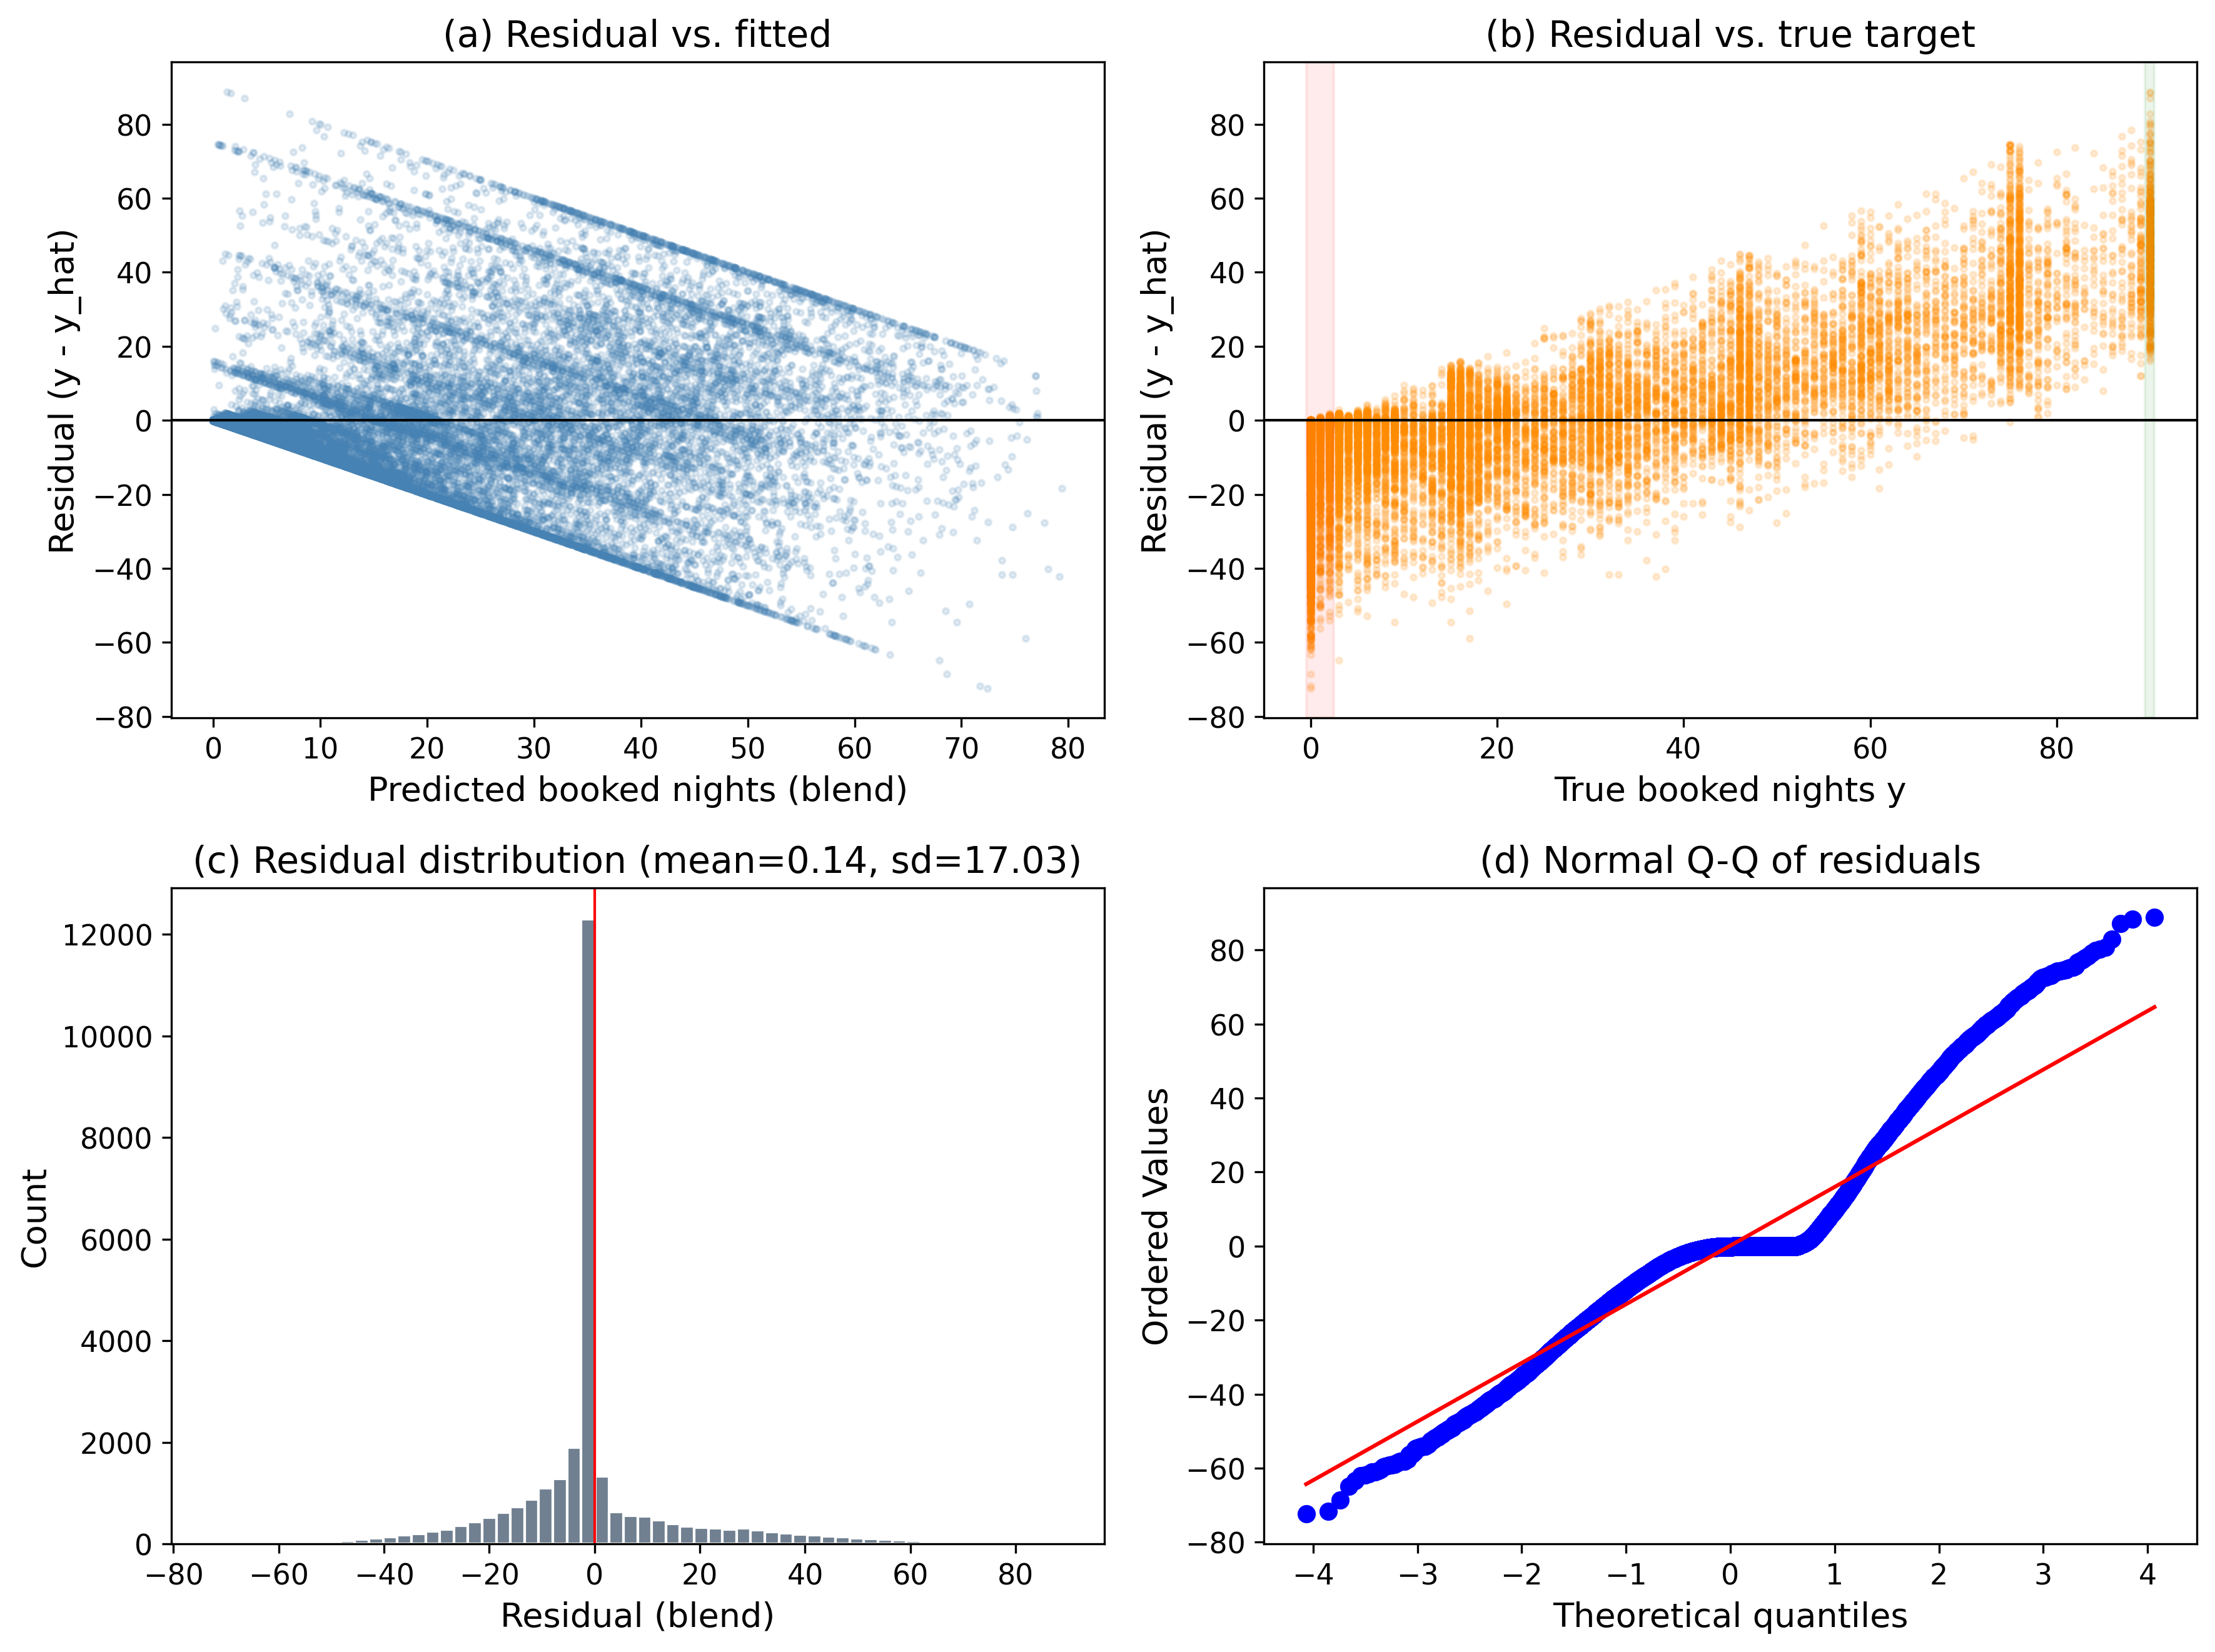
\includegraphics[width=\columnwidth]{fig6_residuals.png}
\caption{Residual diagnostics for the blend on the development OOF predictions:
(a) residual vs.\ fitted, (b) residual vs.\ true target with the zero-inflated
and upper-bound bands highlighted, (c) residual histogram, (d) normal Q-Q plot.}
\label{fig:residuals}
\end{figure}

To localize the bias, the rows are binned by their true value and the mean
signed residual per bin (Fig.~\ref{fig:residualbins}) is plotted. The pattern
is exactly what censoring predicts: for the dead and near-dead listings the
model \emph{over-predicts} (mean residuals of $-4.5$ at $y=0$, $-8.5$ on
$[1,5]$, and $-7.7$ on $[6,20]$, i.e.\ $\hat y>y$), while for the busy listings
it \emph{under-predicts} increasingly toward the bound (mean residual $+3.2$
on $[21,50]$, $+25.9$ on $[51,80]$, $+39.3$ on $[81,89]$, and $+45.5$ at
$y=90$). Clipping to $[0,90]$ removes impossible predictions but does nothing
about this regression-to-the-mean at the boundaries---the estimator shrinks
extreme counts toward the centre of the distribution. This is the clearest
motivation for the two-stage hurdle model implemented next.

\begin{figure}[!t]
\centering
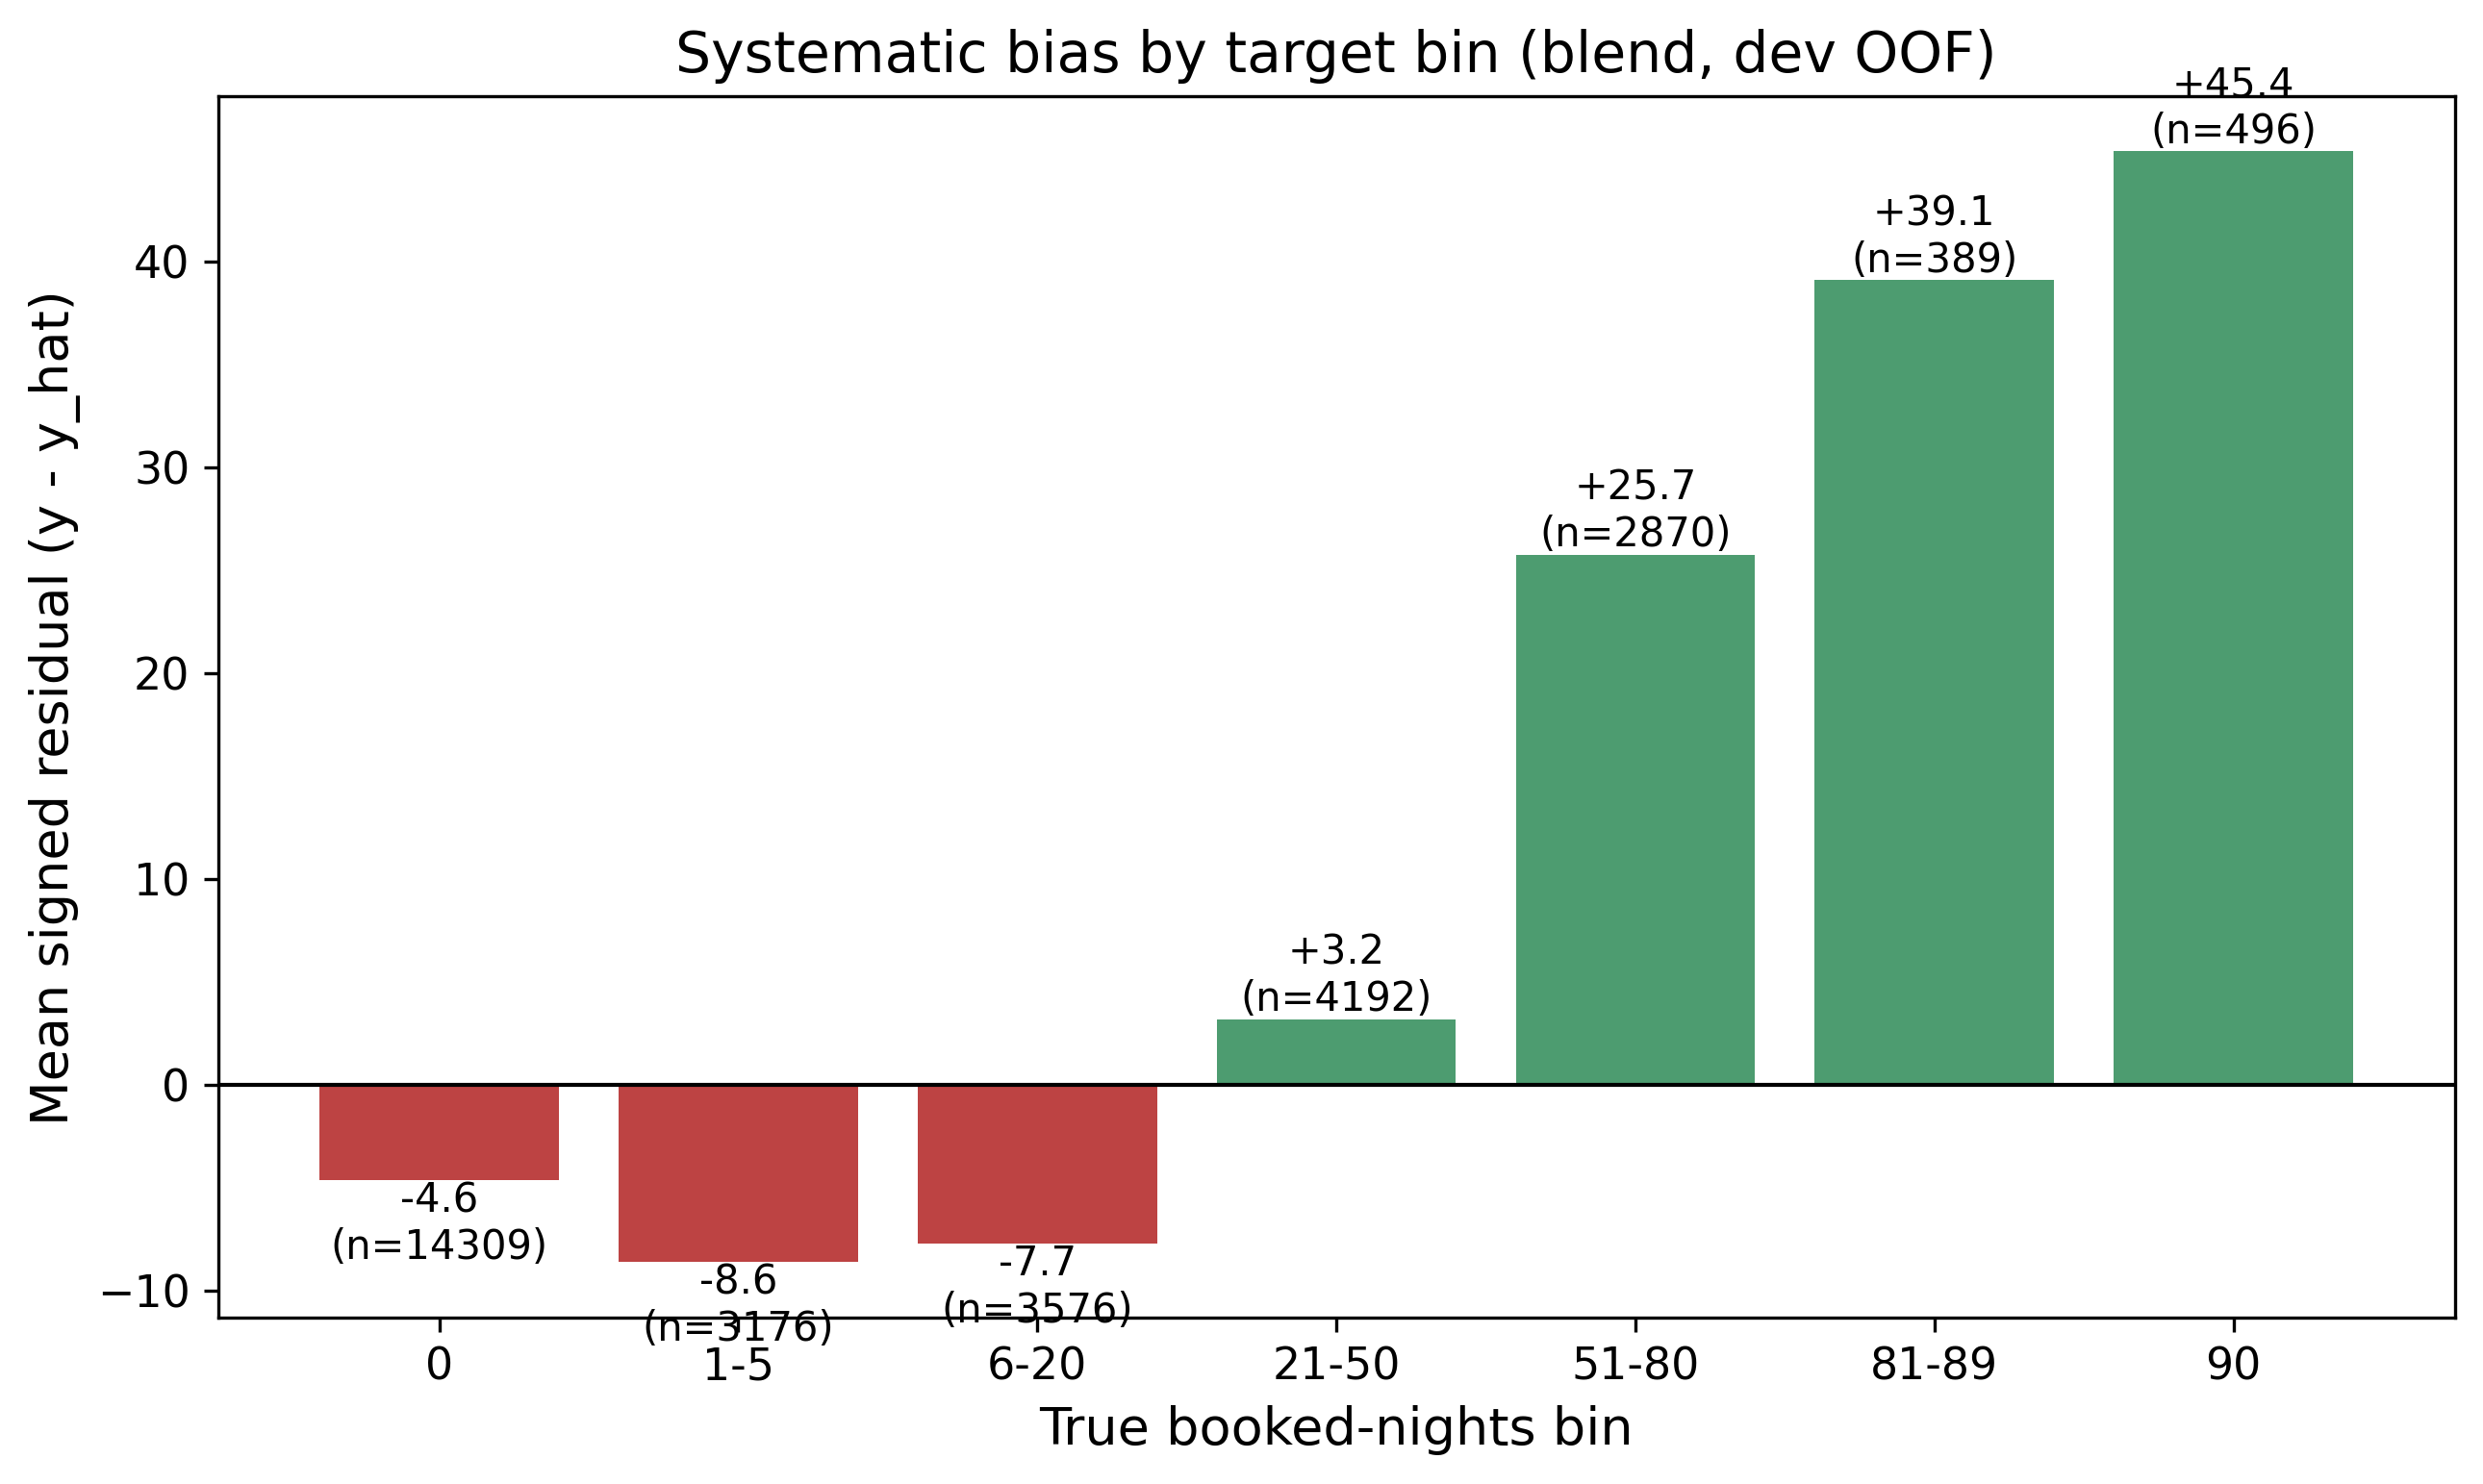
\includegraphics[width=\columnwidth]{fig7_residual_bins.png}
\caption{Mean signed residual ($y-\hat y$) by true booked-nights bin. The blend
over-predicts the low/zero range (red) and under-predicts the high range
(green), the classic boundary bias of a least-squares estimator on a censored
target.}
\label{fig:residualbins}
\end{figure}

\subsection{A Two-Stage Hurdle Model}
\label{sec:hurdle-impl}
Motivated by Section~\ref{sec:zeroinflated} and the boundary bias just
observed, a two-stage hurdle model is implemented rather than only proposed.
For each of XGBoost and LightGBM, a classifier
$p(\mathbf{x})=\Pr(y>0\mid\mathbf{x})$ is fit on the binary label
$\mathbb{1}[y>0]$ over all rows, and a separate regressor
$r(\mathbf{x})=\mathbb{E}[y\mid y>0,\mathbf{x}]$ is fit \emph{only} on the rows
with $y>0$, so it never sees the zeros that drag a single-stage regressor's
predictions down on the $[1,20]$ range (Section~\ref{sec:residuals}). The two
stages factorize the conditional mean as
\begin{equation}
\mathbb{E}[y\mid\mathbf{x}] = \underbrace{\Pr(y>0\mid\mathbf{x})}_{\text{classifier }p(\mathbf{x})}\;\cdot\;\underbrace{\mathbb{E}[y\mid y>0,\mathbf{x}]}_{\text{regressor }r(\mathbf{x})},
\label{eq:hurdle}
\end{equation}
and both stages use the same 5-fold outer split and fold-level early stopping
(a 10\% inner-validation slice per fold) as the rest of the pipeline. The final
prediction is the clipped expected value
$\hat y=\mathrm{clip}\big(p(\mathbf{x})\cdot r(\mathbf{x}),\,0,\,90\big)$.
Table~\ref{tab:hurdle} reports the results. Both hurdle variants alone (298.1
and 299.4 dev MSE) trail the single-stage main XGBoost (295.7), so factorizing
the problem does not automatically help once a well-tuned single-stage model
is already available; but blending the two hurdle expected-value predictions
with the existing nine-model single-stage blend gives a dev MSE of 289.5, a
small further improvement over the single-stage blend's 290.1. On the
held-out local test split the ordering flips by a hair (single-stage blend
286.1 vs.\ hurdle-augmented blend 286.5), so the hurdle model's contribution
is read as a modest, borderline gain rather than a clear win---consistent with
the small effect size already seen for blending
(Section~\ref{sec:significance}), and with the zero-rate of 49.3\% here being
high enough that the single-stage trees already learn a reasonably sharp
implicit decision boundary at $y=0$.

\begin{table}[!t]
\caption{Hurdle model results (development 5-fold CV and held-out local test,
$n_{\text{dev}}=29{,}008$, $n_{\text{test}}=7{,}253$, zero-rate 49.3\%).}
\label{tab:hurdle}
\centering
\begin{tabular}{lcc}
\toprule
Variant & Dev MSE & Test MSE \\
\midrule
Hurdle (XGBoost) & 298.12 & 295.54 \\
Hurdle (LightGBM) & 299.43 & 296.56 \\
Single-stage blend (9 models) & 290.13 & 286.14 \\
\textbf{Hurdle + single-stage blend} & \textbf{289.54} & \textbf{286.54} \\
\bottomrule
\end{tabular}
\end{table}

\subsection{Held-Out Test Performance}
\label{sec:heldout}
The predictions of the nine-model weighted blend are evaluated on the
genuinely held-out local test split (20\% of the data, never touched during
model selection or tuning), where they obtain an MSE of 286.1. This held-out
MSE tracks the internal development CV MSE (290.1) closely; the small gap is
in the direction of \emph{better} test performance, which is plausible given
the larger effective training set used for the final fit and is not a sign of
overfitting. The close agreement between the two numbers indicates that the
cross-validation procedure is honest. For reference, the single best-tuned
XGBoost variant alone scores 288.4 on the same held-out set, so the convex
blend improves the held-out MSE by roughly $0.8\%$ on truly unseen,
future-quarter data, mirroring the out-of-fold gain.

\subsection{Failure-Case Analysis}
\label{sec:failure}
Aggregate metrics and binned residuals describe the model's behaviour
statistically; a sample-level dissection of its worst errors gives
complementary, actionable insight. Table~\ref{tab:failure} lists the
development-set listings with the largest blend under-predictions among
properties blocked at least 80 of the 90 days. Every one of them is a property
close to or at full occupancy ($y=90$) yet predicted at fewer than nine
nights. Their common signature is a near-total absence of a positive-review
track record (0--14 reviews, several with none at all) combined, in two cases,
with a \texttt{recent\_blocking\_rate} of exactly $0$---i.e.\ the H2-2025
recency window shows the listing as \emph{not} recently blocked at all, yet it
is fully booked in Q1 2026. In each case a sudden surge in demand is not
foreshadowed by the historical calendar/review features the model relies on,
so a purely historical regressor cannot anticipate it. Aggregated over the 647
listings with $y\ge88$, the blend predicts a mean of only 45.1 nights despite
a mean \texttt{recent\_blocking\_rate} of 0.92, confirming the systematic
under-prediction near the upper bound. These failures point directly to the
modest gain observed for the hurdle model (Section~\ref{sec:hurdle-impl}) and
to the value of richer demand-acceleration features
(Section~\ref{sec:limitations}).

\begin{table}[!t]
\caption{Largest blend under-predictions among near-fully-booked development
listings ($y\ge90$). Despite near-maximal recent blocking rates, the model
severely under-predicts, as recent behaviour is not corroborated by review
history.}
\label{tab:failure}
\centering
\small
\begin{tabular}{lrrrr}
\toprule
Listing ID & $y$ & $\hat y$ & Recent rate & \#Reviews \\
\midrule
722667459085480621  & 90 & 0.8 & 1.00 & 14 \\
1263194938888022434 & 90 & 1.0 & 0.00 & 0 \\
904891464938130487  & 90 & 2.2 & 1.00 & 0 \\
964806952459028089  & 90 & 6.5 & 1.00 & 0 \\
1406385137935101339 & 90 & 8.0 & 1.00 & 0 \\
\bottomrule
\end{tabular}
\end{table}

\subsection{Threats to Validity}
\label{sec:threats}
This subsection states the main threats to validity. \emph{Internal validity:}
all preprocessing is fitted inside the training fold, target encodings use an
inner $K$-fold (Section~\ref{sec:preproc}), and every feature is built
exclusively from H2-2025 data (Section~\ref{sec:dataset}), so no forward-looking
(2026) information reaches the model as a feature; the held-out local test MSE
(286.1) tracking the development CV MSE (290.1) closely is empirical support
for this. \emph{External validity:} the model is fitted to a single market
(New York City) and a single quarter (Q1 2026), so the learned price and
seasonality effects need not transfer to other cities or years, and the
reliance on H2-2025 calendar-volatility features degrades performance for
brand-new listings with no six-month history (Section~\ref{sec:failure}).
\emph{Construct validity:} the significance test in
Section~\ref{sec:significance} is a paired test on the shared OOF predictions
of the five-model blend rather than a full $5\times2$ cross-validation
\cite{dietterich1998}; it tests the right hypothesis but does not capture
variance from re-drawing the folds themselves, and it was not re-run on the
nine-model blend. Finally, the data-generating process itself changes over an
8-month window (July 2025 to March 2026): any structural shift in the market
between the H2-2025 feature window and the Q1-2026 target window would degrade
real-world performance in a way this fixed train/test split cannot detect.

%==============================================================================
\section{Ablation Study and Migration Notes}
\label{sec:changes}
\label{sec:ablation}
This section isolates the contribution of the proposed components and records
what changed, and what stayed the same, when the pipeline was migrated from a
fixed 2016 Kaggle-cloned-competition snapshot (used in an earlier version of
this study) to the open, continuously-updated Inside Airbnb data.
Table~\ref{tab:ablation} reports a cumulative ablation in which pipeline
components are added one at a time, all measured under the identical 5-fold
cross-validation protocol; the paragraphs that follow analyse the remaining
design choices.

\begin{table}[!t]
\caption{Cumulative ablation (5-fold CV MSE, $\mathtt{random\_state}=42$). The
upper block varies the feature/preprocessing axis with a fixed linear model;
the lower block varies the model/ensemble axis under the full preprocessing.}
\label{tab:ablation}
\centering
\begin{tabular}{lcc}
\toprule
Configuration & MSE & $\Delta$ \\
\midrule
Linear, raw static features only & 384.4 & --- \\
\quad $+$ 206 engineered features (no TE) & 360.2 & $-24.2$ \\
\quad $+$ $K$-fold target encoding (full prep.) & 360.0 & $-0.1$ \\
\midrule
XGBoost (tuned, full prep.) & 295.7 & $-64.3$ \\
Equal-weight blend of 9 learners & 301.0 & $+5.2$ \\
\textbf{SLSQP convex blend (proposed)} & \textbf{290.1} & $-10.8$ \\
\bottomrule
\end{tabular}
\end{table}

\paragraph{Engineered features dominate} The ablation in
Table~\ref{tab:ablation} is unambiguous about where the accuracy comes from.
Adding the 206-column engineered feature matrix to a linear model trained on
the raw static listing fields alone cuts the MSE from 384.4 to 360.2---the
largest single improvement attributable to feature engineering, though modest
in absolute terms next to the model-choice effect below. This confirms that
the calendar/review histories, not the static metadata, carry most of the
predictive signal (Section~\ref{sec:eda}).

\paragraph{Target encoding is close to free on this dataset} Adding the
leakage-safe $K$-fold target encoding of \texttt{neighbourhood\_cleansed}
changes the linear model's MSE only marginally ($360.2\!\rightarrow\!360.0$).
On this dataset the raw categorical carries little signal beyond what the
calendar/recency features already capture, unlike the original 2016 dataset,
where neighbourhood carried more independent price information; the encoding's
main value is representing the high-cardinality field \emph{without leakage}
for the tree models that exploit it (Table~\ref{tab:metrics}), not a direct
accuracy gain for the linear baseline.

\paragraph{Model choice and convex weighting} Switching from the linear model
to the tuned XGBoost under the same preprocessing lowers the MSE by a further
$64.3$ (360.0 to 295.7), confirming the non-linearity argument of
Section~\ref{sec:linearcritique} empirically. The ensemble axis confirms that
naive equal-weight averaging of all nine learners (301.0) is \emph{worse} than
the best single model, because the weaker learners drag the mean down; only
the constrained convex optimisation of \eqref{eq:blendobj}--\eqref{eq:blendbox}
produces a net gain (290.1), by concentrating weight on the complementary
models and assigning zero weight to the redundant learners
(Table~\ref{tab:weights}).

\paragraph{Raw target with clipping beats a log-transform} As in the earlier
2016-data study, training the boosted trees on a log-transformed target
$\log(1+y)$ and inverting at prediction time optimises the wrong objective,
because the evaluation metric is MSE on the raw count scale while the target
is bounded and zero-inflated (Fig.~\ref{fig:target}). Squared error in log
space over-weights the small counts and under-weights the large counts that
dominate the raw MSE. The final XGBoost variants are therefore trained
directly on the raw target with squared-error loss, and the skew is controlled
by clipping predictions to $[0,90]$; the MLP still trains in log space, since
for a gradient-based model the transform is a numerical-stability aid rather
than a change of loss (Section~\ref{sec:mlp}).

\paragraph{Keyword flags suffice; TF-IDF does not help} As before, a TF-IDF
representation of the listing titles does not improve accuracy over simple
keyword flags \cite{islam2022}. Titles are short, so TF-IDF produces a wide,
sparse matrix with little extra signal while increasing overfitting risk and
training time; the compact keyword flags plus title length and word count are
retained, now extended with 14 binary amenity flags parsed from the new
JSON-encoded \texttt{amenities} column.

\paragraph{One raw categorical instead of several} The 2016-data pipeline
target-encoded two high-cardinality columns (neighbourhood and metropolitan
area). Inside Airbnb's schema for this market has one natural analogue,
\texttt{neighbourhood\_cleansed}, kept as a single raw categorical handled
per-fold (Section~\ref{sec:preproc}) rather than flattened into aggregates at
feature-engineering time.

\paragraph{A clean, multi-snapshot target and calendar-volatility features are
new capabilities of this dataset} The 2016 dataset supplied a single
authoritative reservation file for the target quarter, so the target was
unambiguous. Inside Airbnb has no such file, and a single calendar snapshot's
blocked-day count over-counts bookings (Section~\ref{sec:eda}); the target
used here instead requires agreement across at least two of six overlapping
Q1-2026 snapshots. The same repeated re-scraping also makes it possible to
observe, for the training window, how often a listing's recorded availability
flips between consecutive H2-2025 scrapes---the single strongest predictor in
the whole matrix (Section~\ref{sec:results})---with no analogue in a
single-snapshot dataset.

\paragraph{A strict historical-only feature window is a self-imposed
constraint} Because Inside Airbnb is continuously updated rather than a fixed
competition export, nothing enforces a train/test date boundary automatically;
this boundary is imposed explicitly (Section~\ref{sec:dataset}), building every
feature exclusively from H2-2025 and using 2026 data only for the target. This
project-level constraint has no analogue in the original study, where the
competition organizers had already fixed the boundary.

\paragraph{Custom search enables fold-level early stopping} A hand-written
randomized search is used instead of an off-the-shelf cross-validated search
because fold-level early stopping with an \texttt{eval\_set} cannot be
expressed cleanly by the latter. The custom loop preserves the random-sampling
philosophy of \cite{bergstra2012random} and \eqref{eq:searchobj} but
additionally lets each fold stop at its own best iteration
\eqref{eq:earlystop} and logs every trial for inspection; this search is now
applied to five independently-tuned configurations (XGBoost v2/v3, LightGBM,
CatBoost, plus the hand-set main XGBoost as a comparison point,
Section~\ref{sec:tuning}) instead of one, and the SLSQP blend now optimizes
over nine candidate models instead of five (Section~\ref{sec:blend}). A
two-stage hurdle model, only proposed as future work in the earlier study, is
implemented here (Section~\ref{sec:hurdle-impl}).

%==============================================================================
\section{Conclusions}
\label{sec:concl}
This work presented a complete, leakage-safe machine-learning pipeline for
forecasting quarterly short-term-rental demand in New York City from the open
Inside Airbnb data, a censored, zero-inflated regression task under a strict
rule that no feature may be built from information later than the end of the
feature window. From a static listings snapshot and six months of
calendar/review history, 206 per-listing features were engineered; nine model
configurations were compared under 5-fold cross-validation; three boosted-tree
families were independently tuned with an early-stopping randomized search;
the learners were combined through an SLSQP-optimised convex blend; and a
two-stage hurdle model was implemented. The blend attains an out-of-fold MSE of
290.1 and a held-out local test MSE of 286.1, outperforming the best single
model and two state-of-the-art gradient-boosting baselines (LightGBM and
CatBoost); the improvement is statistically significant
(Section~\ref{sec:significance}).

Three findings carry beyond this dataset. Most of the predictive power comes
from calendar histories rather than the static listing table, and specifically
from a feature family (cross-snapshot calendar volatility) that exists only
because the data source re-scrapes the same future dates every month---a
signal with no counterpart in a fixed, single-snapshot dataset. Matching the
loss to the evaluation metric (raw MSE with clipping rather than a
log-transform) matters as much as the choice of learner on a bounded,
zero-inflated target. Finally, a constrained convex blend of complementary
models is a low-cost, low-risk way to obtain a statistically significant
accuracy gain, though an independently-tuned search was found to only match,
not clearly beat, a well-chosen hand-set configuration
(Section~\ref{sec:tuning})---on this feature matrix, the ceiling appears to be
set more by what is fed into the trees than by exact hyper-parameters.

\emph{Scientific and industrial impact.} Accurate quarter-ahead demand
forecasts have concrete value beyond a single benchmark. Platforms can use
booking-density predictions to balance customer-support and infrastructure
capacity ahead of demand peaks, to target marketing toward listings predicted to
be under-booked, and to drive dynamic pricing. At a city scale, booking-density
models can support municipal studies of housing-market pressure and the
displacement of long-term rental stock by short-term lets. The methodological
contribution---formalised leakage-safe target encoding combined with a
constrained convex ensemble and an implemented hurdle extension for a censored,
zero-inflated target, all under a strict historical-only feature constraint---
transfers to other bounded count-forecasting problems such as occupancy,
attendance, or inventory demand.

\subsection{Limitations and Future Work}
\label{sec:limitations}
Several limitations bound the present results and motivate future work.
\emph{Geographic and temporal specificity:} the model is fitted to a single
market (New York City) and a single quarter (Q1 2026), so the learned price and
seasonality effects need not transfer to other cities or years.
\emph{Cold-start dependence:} predictions rely heavily on H2-2025 calendar
history, so accuracy degrades for brand-new listings, which is the dominant
failure mode identified in Section~\ref{sec:failure}.
\emph{Search cost:} the customised fold-level randomized search is inherently
more sequential than a fully parallelised grid search, trading wall-clock
efficiency for the ability to apply per-fold early stopping.
\emph{Static quarterly horizon:} the formulation predicts a single quarterly
aggregate and does not capture dynamic, week-to-week variation in booking
behaviour. \emph{Untested temporal generalization:} unlike a fixed competition
snapshot, this open dataset could in principle be used to validate the
pipeline against a later quarter (e.g.\ Q2 2026) as it becomes available, but
that validation has not yet been performed.

Future work follows directly from these limitations, from the residual
analysis (Section~\ref{sec:residuals}), and from the hurdle model's only
borderline gain (Section~\ref{sec:hurdle-impl}). First, the hurdle classifier
and regressor currently draw only on XGBoost and LightGBM; letting them share
the blend's full nine-model diversity might close more of the boundary bias in
Fig.~\ref{fig:residualbins}. Second, richer trajectory features---for example a
longer or more flexible fit than the current short linear trend---would better
separate listings whose demand is \emph{accelerating} from those merely busy on
average, directly targeting the failure cases in Section~\ref{sec:failure}.
Third, because the MLP is the learner least correlated with the tree ensembles
(Table~\ref{tab:errcorr}), a more careful neural-network search is a promising
route to a stronger blend partner. Finally, re-running the pipeline against a
subsequent Inside Airbnb scrape, once a later quarter's outcome is known, would
be a direct, non-simulated test of the external-validity concerns raised in
Section~\ref{sec:threats}.

%==============================================================================
\bibliographystyle{IEEEtran}
\bibliography{references}

%==============================================================================
\appendices
\section{Reproducibility and Execution Environment}
\label{app:env}
All results are reproducible from a single fixed seed
(\texttt{random\_state}~$=42$), which governs the 80/20 development/hold-out
split, the 5-fold cross-validation partitions, the inner target-encoding folds,
and the random-search samplers. The pipeline is implemented in Python~3.14
with scikit-learn~1.8.0 (preprocessing, linear, random-forest and
gradient-boosting models, cross-validation), XGBoost~3.2.0, PyTorch~2.12 (CPU
build) with Adam for the MLP, SciPy~1.17.1 for the SLSQP blend, and
LightGBM~4.6.0 and CatBoost~1.2.10 for the external baselines. All experiments
were run on a single workstation with no GPU. Representative wall-clock times
per hyper-parameter configuration (5-fold CV, fold-level early stopping) are:
XGBoost v2 $\approx$64\,s (30-configuration search $\approx$32\,min); XGBoost
v3 $\approx$49\,s (60-configuration search $\approx$49\,min); CatBoost
$\approx$40\,s (40-configuration search $\approx$27\,min); LightGBM
$\approx$530\,s (40-configuration search $\approx$5.9\,h, markedly the most
expensive stage of the pipeline given its larger tree/leaf budget in this
search); and the SLSQP blend $<$1\,s regardless of the number of candidate
models. Out-of-fold predictions are cached to disk so that the blend and all
post-hoc diagnostics can be recomputed without retraining.

\section{Engineered Feature Inventory}
\label{app:features}
Table~\ref{tab:featinventory} documents the 206 engineered columns (205
numeric, 1 raw categorical) by family, with their source tables and a
representative mathematical definition, so that the feature matrix can be
reproduced. Per-quarter aggregates are computed independently for Q3, Q4, and
the combined second half (H2) of 2025; rates are normalised by the number of
days a listing is observed in the period.

\begin{table}[!t]
\caption{Engineered feature families, source tables, and representative
definitions. ``calendar'' denotes the H2-2025 monthly calendar files;
``static'' denotes the December-2025 listings snapshot. $\mathbb{1}[\cdot]$ is
the indicator function.}
\label{tab:featinventory}
\centering
\footnotesize
\begin{tabular}{p{1.05in}p{0.45in}p{1.25in}}
\toprule
Family (source) & \# & Representative definition \\
\midrule
Per-quarter/H2 aggregates (calendar) & 41 & blocking rate $=\frac{\#\{\text{blocked days}\}}{\#\{\text{observed days}\}}$ \\
Monthly rates \& transitions (calendar) & 6 & $\sum_{d\in\text{month}}\mathbb{1}[\text{available}_d{=}\text{f}]$ \\
Recency \& trajectory (calendar) & 20 & least-squares slope of recent blocking rate \\
Cross-snapshot volatility (calendar) & 3 & $\#\{d:\text{avail}_d^{(t)}\ne\text{avail}_d^{(t-1)}\}$ \\
Price / revenue (calendar+static) & 8 & $\mathrm{CV}_p=\sigma_{p}/\mu_{p}$; \texttt{estimated\_revenue\_l365d} \\
Reviews (static) & 13 & counts over 30/90/180/365d; 90d acceleration \\
Property/host metadata (static) & 32 & accommodates; bedrooms; host tenure; missing-indicators \\
Text keywords / amenities (static) & 24 & $\mathbb{1}[\text{title contains ``luxury''}]$; JSON amenity flags \\
Geographic / neighbourhood (static) & 27 & K-Means$(k{=}19)$ cluster of (lat, lon); nbhd context \\
\bottomrule
\end{tabular}
\end{table}


\section{Complete Feature Inventory}
\label{app:allfeatures_table}
Here is the complete inventory of all 206 engineered feature columns, along
with the identifier and target variables and their corresponding data types.
Three columns (\texttt{estimated\_revenue\_l365d}, \texttt{price\_implied},
\texttt{implied\_nightly\_rate}) are retained for pipeline/schema consistency
with the original 2016-data feature set but are 100\% missing in this Inside
Airbnb export (Section~\ref{sec:eda}) and are median-imputed to a constant like
any other missing column.

\begin{table*}[!ht]
\caption{Detailed list of all 208 columns in the processed feature matrix
(identifier, target, and 206 features).}
\label{tab:allfeatures_list}
\centering
\footnotesize
\begin{tabular}{ll|ll|ll}
\toprule
Feature Name & Type & Feature Name & Type & Feature Name & Type \\
\midrule
\texttt{id} & integer (ID) & \texttt{blocked\_days\_Q1\_2026} & integer (target) & \texttt{q3\_days\_total} & float \\
\texttt{q3\_days\_blocked} & float & \texttt{q3\_days\_avail} & float & \texttt{q3\_blocking\_rate} & float \\
\texttt{q3\_avail\_rate} & float & \texttt{q3\_we\_blocking\_rate} & float & \texttt{q3\_we\_days} & float \\
\texttt{q3\_wd\_blocking\_rate} & float & \texttt{q3\_wd\_days} & float & \texttt{q3\_new\_blockings} & float \\
\texttt{q3\_new\_unblockings} & float & \texttt{q3\_we\_minus\_wd\_blocking} & float & \texttt{q4\_days\_total} & integer \\
\texttt{q4\_days\_blocked} & integer & \texttt{q4\_days\_avail} & integer & \texttt{q4\_blocking\_rate} & float \\
\texttt{q4\_avail\_rate} & float & \texttt{q4\_we\_blocking\_rate} & float & \texttt{q4\_we\_days} & integer \\
\texttt{q4\_wd\_blocking\_rate} & float & \texttt{q4\_wd\_days} & integer & \texttt{q4\_new\_blockings} & integer \\
\texttt{q4\_new\_unblockings} & integer & \texttt{q4\_we\_minus\_wd\_blocking} & float & \texttt{h2\_days\_total} & integer \\
\texttt{h2\_days\_blocked} & integer & \texttt{h2\_days\_avail} & integer & \texttt{h2\_blocking\_rate} & float \\
\texttt{h2\_avail\_rate} & float & \texttt{h2\_we\_blocking\_rate} & float & \texttt{h2\_we\_days} & integer \\
\texttt{h2\_wd\_blocking\_rate} & float & \texttt{h2\_wd\_days} & integer & \texttt{h2\_new\_blockings} & integer \\
\texttt{h2\_new\_unblockings} & integer & \texttt{h2\_we\_minus\_wd\_blocking} & float & \texttt{m7\_blocking\_rate} & float \\
\texttt{m7\_days} & float & \texttt{m8\_blocking\_rate} & float & \texttt{m8\_days} & float \\
\texttt{m9\_blocking\_rate} & float & \texttt{m9\_days} & float & \texttt{m10\_blocking\_rate} & float \\
\texttt{m10\_days} & float & \texttt{m11\_blocking\_rate} & float & \texttt{m11\_days} & float \\
\texttt{m12\_blocking\_rate} & float & \texttt{m12\_days} & float & \texttt{recent\_days\_total} & integer \\
\texttt{recent\_days\_blocked} & integer & \texttt{recent\_days\_avail} & integer & \texttt{recent\_blocking\_rate} & float \\
\texttt{recent\_avail\_rate} & float & \texttt{recent\_we\_blocking\_rate} & float & \texttt{recent\_we\_days} & integer \\
\texttt{recent\_wd\_blocking\_rate} & float & \texttt{recent\_wd\_days} & integer & \texttt{recent\_new\_blockings} & integer \\
\texttt{recent\_new\_unblockings} & integer & \texttt{recent\_we\_minus\_wd\_blocking} & float & \texttt{h2\_flips} & integer \\
\texttt{h2\_multi\_obs\_days} & integer & \texttt{h2\_flip\_rate} & float & \texttt{hosts\_time\_as\_user\_years} & float \\
\texttt{hosts\_time\_as\_user\_months} & float & \texttt{hosts\_time\_as\_host\_years} & float & \texttt{hosts\_time\_as\_host\_months} & float \\
\texttt{host\_listings\_count} & float & \texttt{host\_total\_listings\_count} & float & \texttt{neighbourhood\_cleansed} & str (raw cat.) \\
\texttt{latitude} & float & \texttt{longitude} & float & \texttt{accommodates} & float \\
\texttt{bedrooms} & float & \texttt{beds} & float & \texttt{minimum\_nights} & float \\
\texttt{maximum\_nights} & float & \texttt{minimum\_minimum\_nights} & float & \texttt{maximum\_minimum\_nights} & float \\
\texttt{minimum\_maximum\_nights} & float & \texttt{maximum\_maximum\_nights} & float & \texttt{minimum\_nights\_avg\_ntm} & float \\
\texttt{maximum\_nights\_avg\_ntm} & float & \texttt{number\_of\_reviews} & float & \texttt{number\_of\_reviews\_ltm} & float \\
\texttt{number\_of\_reviews\_l30d} & float & \texttt{number\_of\_reviews\_ly} & float & \texttt{estimated\_occupancy\_l365d} & float \\
\texttt{estimated\_revenue\_l365d} & float (all-missing) & \texttt{review\_scores\_rating} & float & \texttt{review\_scores\_accuracy} & float \\
\texttt{review\_scores\_cleanliness} & float & \texttt{review\_scores\_checkin} & float & \texttt{review\_scores\_communication} & float \\
\texttt{review\_scores\_location} & float & \texttt{review\_scores\_value} & float & \texttt{calculated\_host\_listings\_count} & float \\
\texttt{calculated\_host\_listings\_count\_entire\_homes} & integer & \texttt{calculated\_host\_listings\_count\_private\_rooms} & integer & \texttt{calculated\_host\_listings\_count\_shared\_rooms} & integer \\
\texttt{reviews\_per\_month} & float & \texttt{p5\_mean} & float & \texttt{p5\_std} & float \\
\texttt{p5\_cv} & float & \texttt{p5\_trend} & float & \texttt{p5\_min} & float \\
\texttt{p5\_max} & float & \texttt{p5\_range} & float & \texttt{p5\_n\_distinct} & float \\
\texttt{price\_implied} & float (all-missing) & \texttt{price\_numeric} & float & \texttt{price\_missing} & binary \\
\texttt{price\_rel\_nbhd} & float & \texttt{host\_response\_rate\_num} & float & \texttt{host\_acceptance\_rate\_num} & float \\
\texttt{host\_is\_superhost\_enc} & binary & \texttt{instant\_bookable\_enc} & binary & \texttt{host\_identity\_verified\_enc} & binary \\
\texttt{host\_has\_profile\_pic\_enc} & binary & \texttt{host\_response\_time\_enc} & float & \texttt{host\_response\_time\_missing} & binary \\
\texttt{host\_age\_days} & float & \texttt{listing\_age\_days} & float & \texttt{days\_since\_last\_review} & float \\
\texttt{has\_reviews} & binary & \texttt{price\_per\_guest} & float & \texttt{min\_stay\_x\_price} & float \\
\texttt{implied\_nightly\_rate} & float (all-missing) & \texttt{bathrooms\_num} & float & \texttt{bath\_is\_shared} & binary \\
\texttt{amen\_wifi} & binary & \texttt{amen\_kitchen} & binary & \texttt{amen\_ac} & binary \\
\texttt{amen\_washer} & binary & \texttt{amen\_dryer} & binary & \texttt{amen\_parking} & binary \\
\texttt{amen\_elevator} & binary & \texttt{amen\_tv} & binary & \texttt{amen\_pool} & binary \\
\texttt{amen\_gym} & binary & \texttt{amen\_co\_alarm} & binary & \texttt{amen\_long\_term} & binary \\
\texttt{amen\_self\_checkin} & binary & \texttt{amen\_hot\_tub} & binary & \texttt{kw\_luxury} & binary \\
\texttt{kw\_private} & binary & \texttt{kw\_cozy} & binary & \texttt{kw\_modern} & binary \\
\texttt{kw\_view} & binary & \texttt{kw\_near} & binary & \texttt{kw\_spacious} & binary \\
\texttt{kw\_studio} & binary & \texttt{title\_len} & integer & \texttt{title\_words} & integer \\
\texttt{property\_type\_grp\_Hotel\_Hostel} & binary & \texttt{property\_type\_grp\_Other} & binary & \texttt{property\_type\_grp\_Private\_Room} & binary \\
\texttt{property\_type\_grp\_Shared\_Room} & binary & \texttt{room\_type\_Hotel room} & binary & \texttt{room\_type\_Private room} & binary \\
\texttt{room\_type\_Shared room} & binary & \texttt{neighbourhood\_group\_cleansed\_Brooklyn} & binary & \texttt{neighbourhood\_group\_cleansed\_Manhattan} & binary \\
\texttt{neighbourhood\_group\_cleansed\_Queens} & binary & \texttt{neighbourhood\_group\_cleansed\_Staten Island} & binary & \texttt{neighbourhood\_freq} & float \\
\texttt{geo\_cluster\_1} & binary & \texttt{geo\_cluster\_2} & binary & \texttt{geo\_cluster\_3} & binary \\
\texttt{geo\_cluster\_4} & binary & \texttt{geo\_cluster\_5} & binary & \texttt{geo\_cluster\_6} & binary \\
\texttt{geo\_cluster\_7} & binary & \texttt{geo\_cluster\_8} & binary & \texttt{geo\_cluster\_9} & binary \\
\texttt{geo\_cluster\_10} & binary & \texttt{geo\_cluster\_11} & binary & \texttt{geo\_cluster\_12} & binary \\
\texttt{geo\_cluster\_13} & binary & \texttt{geo\_cluster\_14} & binary & \texttt{geo\_cluster\_15} & binary \\
\texttt{geo\_cluster\_16} & binary & \texttt{geo\_cluster\_17} & binary & \texttt{geo\_cluster\_18} & binary \\
\texttt{geo\_cluster\_19} & binary & \texttt{rev\_30d} & integer & \texttt{rev\_90d} & integer \\
\texttt{rev\_180d} & integer & \texttt{rev\_365d} & integer & \texttt{rev\_accel\_90} & integer \\
\texttt{q3\_to\_q4\_blocking\_trend} & float & \texttt{q3\_to\_q4\_blocking\_ratio} & float & \texttt{recent\_fully\_blocked} & binary \\
\texttt{traj\_slope} & float & \texttt{traj\_recent3} & float & \texttt{traj\_older3} & float \\
\texttt{traj\_recent\_older\_ratio} & float & \texttt{traj\_accel} & float & \texttt{traj\_std} & float \\
\texttt{traj\_nonzero\_months} & integer & \texttt{nb\_mean\_rate} & float & \texttt{nb\_density} & integer \\
\texttt{rate\_vs\_nb} & float & \texttt{geo\_mean\_rate} & float & \texttt{geo\_density} & integer \\
\texttt{rate\_vs\_geo} & float &  &  &  &  \\
\bottomrule
\end{tabular}
\end{table*}

\end{document}
